\documentclass[12pt,letterpaper]{article}
\usepackage[a4paper, total={7in, 10in}]{geometry}
\renewcommand{\familydefault}{\sfdefault}
\usepackage{graphicx}
\usepackage{helvet}
\usepackage{authblk}
\usepackage{hyperref}
\usepackage{amsmath} 
\usepackage{amssymb} 
\usepackage{orcidlink} 
\usepackage[super,comma,sort&compress]  
   {natbib}\bibliographystyle{numbered}
% \usepackage[right]{lineno} \linenumbers


\makeatletter
\renewcommand{\maketitle}{\bgroup\setlength{\parindent}{0pt}
\begin{flushleft}
  \textbf{\@title}
  
  \@author
\end{flushleft}\egroup}
\makeatother

%%%  Insert title below; leave date empty.

\title{Deciphering enhancer rules underlying early human neuronal and neural crest development.}
\date{}

%%%  Author first and last names should be spelled 
%%%  out in their entirety (do not abbreviate "J.H. 
%%%  Watson" unless this is how the author's name 
%%%  always appears). Middle initials are OK. Do 
%%%  not include titles, positions, or degrees.

%%%  Use numbered footnotes to indicate institutional 
%%%  affiliations. Authors may have multiple 
%%%  institutional affiliations, and affiliations 
%%%  may be shared among multiple authors.

%%%  After the institutional affiliations, numbered 
%%%  footnotes may be used to indicate an author's 
%%%  present address, equal contribution status, 
%%%  and/or senior author status. Corresponding 
%%%  authors may additionally include Twitter (X) 
%%%  handles as a means of contact.

%%%  The final numbered footnote should indicate 
%%%  which author is the lead contact (required). 
%%%  One author must be designated as the lead contact. 
%%%  There can be no more than one lead contact. 

%%%  Corresponding authors should be indicated with 
%%%  asterisks (*). Use 2 asterisks (**) for the 
%%%  second-listed corresponding author, 3 (***) for 
%%%  the third-listed, and so on. The lead contact 
%%%  must be a corresponding author. Additional 
%%%  authors may also serve as corresponding authors.

\author[1,2,3,\orcidlink{0000-0001-7907-1247}]{Seppe De Winter}
\author[1,2,3,*,\orcidlink{0000-0002-8006-0315}]{Stein Aerts}


%%%  Institutional affiliations should contain the 
%%%  following information at minimum: department(s)/
%%%  subunit(s), institution, city, state/region (if 
%%%  applicable), and country. 

\affil[1]{VIB Center of AI \& computational Biology, Leuven, Belgium}
\affil[2]{VIB-KU Leuven Center for Brain and Disease Research, Leuven, Belgium}
\affil[3]{KU Leuven Department of Human Genetics, Leuven, Belgium}

%%%  List only one email address per corresponding author.

\affil[*]{Correspondence: stein.aerts@kuleuven.be}


\begin{document}

\maketitle

\section*{SUMMARY}

%%% The summary (abstract) should consist of a single paragraph of 150 words or fewer.

\section*{KEYWORDS}

%%%  Include up to 10 keywords, separated by commas. 
%%%  Keywords entered in EM are not carried over; only 
%%%  keywords included in the main text will be used 
%%%  in the final article metadata. Please note that 
%%%  for some journals, keywords are chosen by the editors.

\section*{INTRODUCTION}

%%% INTRO TO FIELD

Genomes of complex multi-cellular organisms encode all cell types/states\cite{trapnellDefiningCellTypes2015, arendtOriginEvolutionCell2016, fleckWhatCellType2023} of that organism in specific non-coding elements named
enhancers\cite{davidsonRegulatoryGenomeGene2010}. The code words used by enhancers are
transcription factor binding sites (TFBS)\cite{davidsonRegulatoryGenomeGene2010} and the precise arrangement, copy
number and strength of individual TFBS define the enhancer and its cell type-specific activity\cite{dewinterModellingDesignTranscriptional2025}. Due to the soft syntax rules underlying the enhancer-code\cite{zeitlingerSevenMythsHow2020}, DNA sequence based deep learning methods have shown major advances in the ability to model and explain enhancers\cite{zeitlingerSevenMythsHow2020, dewinterModellingDesignTranscriptional2025}. For example, during immune cell differentiation\cite{maslovaDeepLearningImmune2020}, fly brain cell types\cite{janssensDecodingGeneRegulation2022}, liver cell types\cite{bravogonzalez-blasSinglecellSpatialMultiomics2024}, melanoma states\cite{minnoyeCrossspeciesAnalysisEnhancer2020, atakInterpretationAllelespecificChromatin2021}, during human brain development\cite{mannensChromatinAccessibilityHuman2024}, mammalian and chicken brain cell types\cite{heckerEnhancerdrivenCellType2025} and pluripotent cell stem cells\cite{avsecBaseresolutionModelsTranscriptionfactor2021}. Furthermore, it has been demonstrated recently that the code learned by these models is sufficient to design novel enhancers with cell type-specific activity\cite{taskiranCelltypedirectedDesignSynthetic2024, dealmeidaTargetedDesignSynthetic2024, gosaiMachineguidedDesignCelltypetargeting2024, yinIterativeDeepLearningdesign2024}.\par

Organoids are a reductionistic biological model system that can be used to interrogate how cell types are encoded in the
genome. Especially organoids derived from pluripotent stem cells are interesting in this context, given that they
demonstrate how a single genome can generate multiple distinct cell types\cite{mccauleyPluripotentStemCellderived2017,
takebeOrganoidsDesign2019, hoferEngineeringOrganoids2021}. Organoids can furthermore, give insights into how genomes
interpret both cell intrinsic and extrinsic signals. For example, epigentic
modifications\cite{zenkSinglecellEpigenomicReconstruction2024}, transcription factor (TF)
perturbations\cite{fleckInferringPerturbingCell2023} or morphogen
signaling\cite{sanchis-callejaDecodingMorphogenPatterning2024}. Another benefit of organoids is that they can be used to
model biological systems that are otherwise - due to ethical and/or practical reasons - inaccessible for study. For
example, early human development.\par

%%% What is missing and bridge

Current efforts are ongoing to determine the breadth of human cell types that can be generated using organoid protocols and how they compare to their primary counterparts, at a transcriptomic level. For example, for brain organoids\cite{heIntegratedTranscriptomicCell2024} and endoderm-derived organoids\cite{xuIntegratedTranscriptomicCell2023}. However, such comparisons at the level of the enhancer-code are still limited\cite{zenkSinglecellEpigenomicReconstruction2024, fleckInferringPerturbingCell2023}.\par

During vertebrate development both the neural tube and neural crest originate from the neural ectoderm. The neural tube
consist of proliferating neuronal progenitors that, through opposing gradients of SHH and BMP/Wnt signaling, have different identities along the dorso-ventral (DV) axis of the embryo later giving rise to distinct neuronal subtypes of the central nervous system\cite{sagnerEstablishingNeuronalDiversity2019, delasRepressiveInteractionsGene2020}. Neural crest cells originate from the neural plate border, through intermediate signals of BMP and Wnt\cite{simoes-costaEstablishingNeuralCrest2015}, and migrate throughout the body giving rise to a multitude of cell types including the peripheral nervous system, craniofacial skeleton and melanocytes\cite{simoes-costaEstablishingNeuralCrest2015}. The gene regulatory networks underlying both DV patterning of neuronal progenitors\cite{sagnerEstablishingNeuronalDiversity2019, delasRepressiveInteractionsGene2020} and neural crest induction, specification, migration and differentiation\cite{simoes-costaEstablishingNeuralCrest2015, candido-ferreiraMultilayeredTranscriptionalControl2023} are already well studied. Furthermore, studies using chromatin accessibility profiling methods at the bulk and single cell level, profiling enhancers encoding cell types and states of neuronal progenitors and neural crest cells are starting to emerge\cite{delasDevelopmentalCellFate2023, zhangCisregulatoryLogicIntegrating2024, huEndothelialRegulatoryCircuits2025} but a detailed descriptions of the enhancer-code of each individual cell types are still limited.\par

In this study, we will determine the enhancer-codes of cell types/states generated by human neural tube organoids, a model system for early human neuronal and neural crest development\cite{abdelfattahActuationEnhancesPatterning2021} and compare these codes to those of cell types/states of the head of a four weeks post conception human embryo.


\section*{RESULTS}

\subsection*{Human neural tube organoids recapitulate early neuronal and neural crest development}
We made use of human neural tube organoids (hNTOs) to model early human neuronal and neural crest development. To this
end we embedded single cells from two induced pluripotent stem cell (iPSC) lines (Sigma and BJ1) and one embryonic stem
cell line (ESC; H9) into separate synthetic poly-ethylene glycol (PEG) based extracellular matrices. These were
incubated for 11 days and we supplemented the medium with retinoic acid (RA) and Smoothened agonist (SAG) from day 3
until day 5 (\textbf{Fig. 1a}). These conditions were previously shown to generate multiple neuronal progenitor and
neural crest states (REF). In order to characterize the organoid-derived cell types to a greater level of detail at both
transcriptomic as well as chromatin accessibility level we performed 10x single-cell multiomics (combined scATAC-seq and
scRNA-seq) at four time points of differentiation (day 4-5, day 6-7, day 8-9 and day 10-110; \textbf{Fig. 1a}),
resulting in 22,862 high quality cells (\textbf{Fig. 1b}). Note, that similar transcriptomic and chromatin accessibility
states were obtained from all three cell lines (\textbf{FIGURE SUPPLEMENT}) demonstrating the robustness of the
organoid system.\par
To evaluate the biological relevance of the cell types and states obtained from the organoid, we performed 10x single
cell multiome on the head of a single four weeks post conception human embryo, resulting in 25,785 high quality cells (
\textbf{Fig. 1c}). We annotated both the organoid and embryo cells based on the expression of marker genes
(\textbf{TABLE SUPPLEMENT}). In both systems we could identify neuronal progenitor cells, early differentiating neurons,
neural crest cells, facial mesenchyme cells and early differentiating peripheral neurons (\textbf{Fig. 1b-c}).
Additionally, in the organoid only we could identify a pluripotent stem cell population (\textbf{Fig. 1b}) and in the
embryo only we could identify an endothelial, perivascular macrophage (PVM) / microglia (MIC) and otic placode
population (\textbf{Fig. 1c}).\par
Next, we sub-clustered the neuronal progenitor, early neuron, and neural crest cell types (\textbf{Fig. 1d-f}). Both
organoid and embryo neuronal progenitors show a gradient of different cell states reflecting dorso-ventral patterning as
is evident from the expression of dorso-ventral marker TFs (REF): from ventral to dorsal ARX, NKX2-2, PAX6, IRX3, ZIC1 and
GDF7 (\textbf{Fig. 1d}). In both the organoid and embryo system we obtained multiple early neuronal differentiation states.
A cluster that still expresses the neuronal progenitor marker SOX2, cells that express the early neuronal induction
marker ASCL1 and distinct clusters marked by the expression of GAD1, UNCX and GATA2 (\textbf{Fig. 1e}). Finally,
focusing on the neural crest cells, in both the organoid and the embryo we obtained a population of pre-migratory neural
crest (GRHL2 expression and absence of ZEB2 expression), migratory neural crest (SOX10 and ZEB2 expression), facial
mesenchyme cells (TWIST1 expression) and early differentiation peripheral neurons (NEUROD1 expression). In the embryo,
but not in the organoid, we observed an additional population of cells marked by the expression of SOX10 and PAX2
reflecting the otic placode (\textbf{Fig. 1f}).\par
Given that we performed single-cell multiome on the entire head of the four weeks post conception embryo we also
assessed the expression of anterior-posterior marker TFs. While the organoid cells had either an anterior forebrain
(SIX3) or anterior spinal cord (HOXB3) identity, we observed a gradient of anterior-to-posterior identities in the
embryo (REF): from anterior to posterior expression of SIX3, EMX2, FOXG1, BARHL1, EN1 and HOXB3 (\textbf{Fig. 1g}).\par
Cell cycle arrest is an important hallmark of the start of neuronal differentiation (REF), for this reason we scored
both organoid and embryo cells for the expression of marker genes of the G1, G2M and S phase of the cell cycle and
quantified the fraction of cells in each phase stratified by the main cell types (\textbf{Fig. 1h}). From this it is
clear that both early differentiation peripheral neurons and to a greater extend early differentiating neurons of the
central nervous system are in cell cycle arrest, while the other cell types are still cycling (\textbf{Fig. 1h}).\par
Finally, to assess whether the organoid-derived cell types and states are also similar to the embryo-derived cell types
and states on a chromatin accessibility level we identified sets of co-accessible regions in the organoid model using
topic modeling. We focused on topics (i.e., sets of co-accessible regions) that were enriched for marker TF motifs and
calculated the average expression of marker genes for each cell group where these regions were co-accessible, for both
organoid and embryo cells. We observed similar patterns of marker gene expression for the same cell state (defined by
the topic) across the organoid and embryo (\textbf{Fig. 1i}) with an average Pearson correlation coefficient of \textbf{X.X}
across identical states (\textbf{FIGURE SUPPLEMENT}).\par

\noindent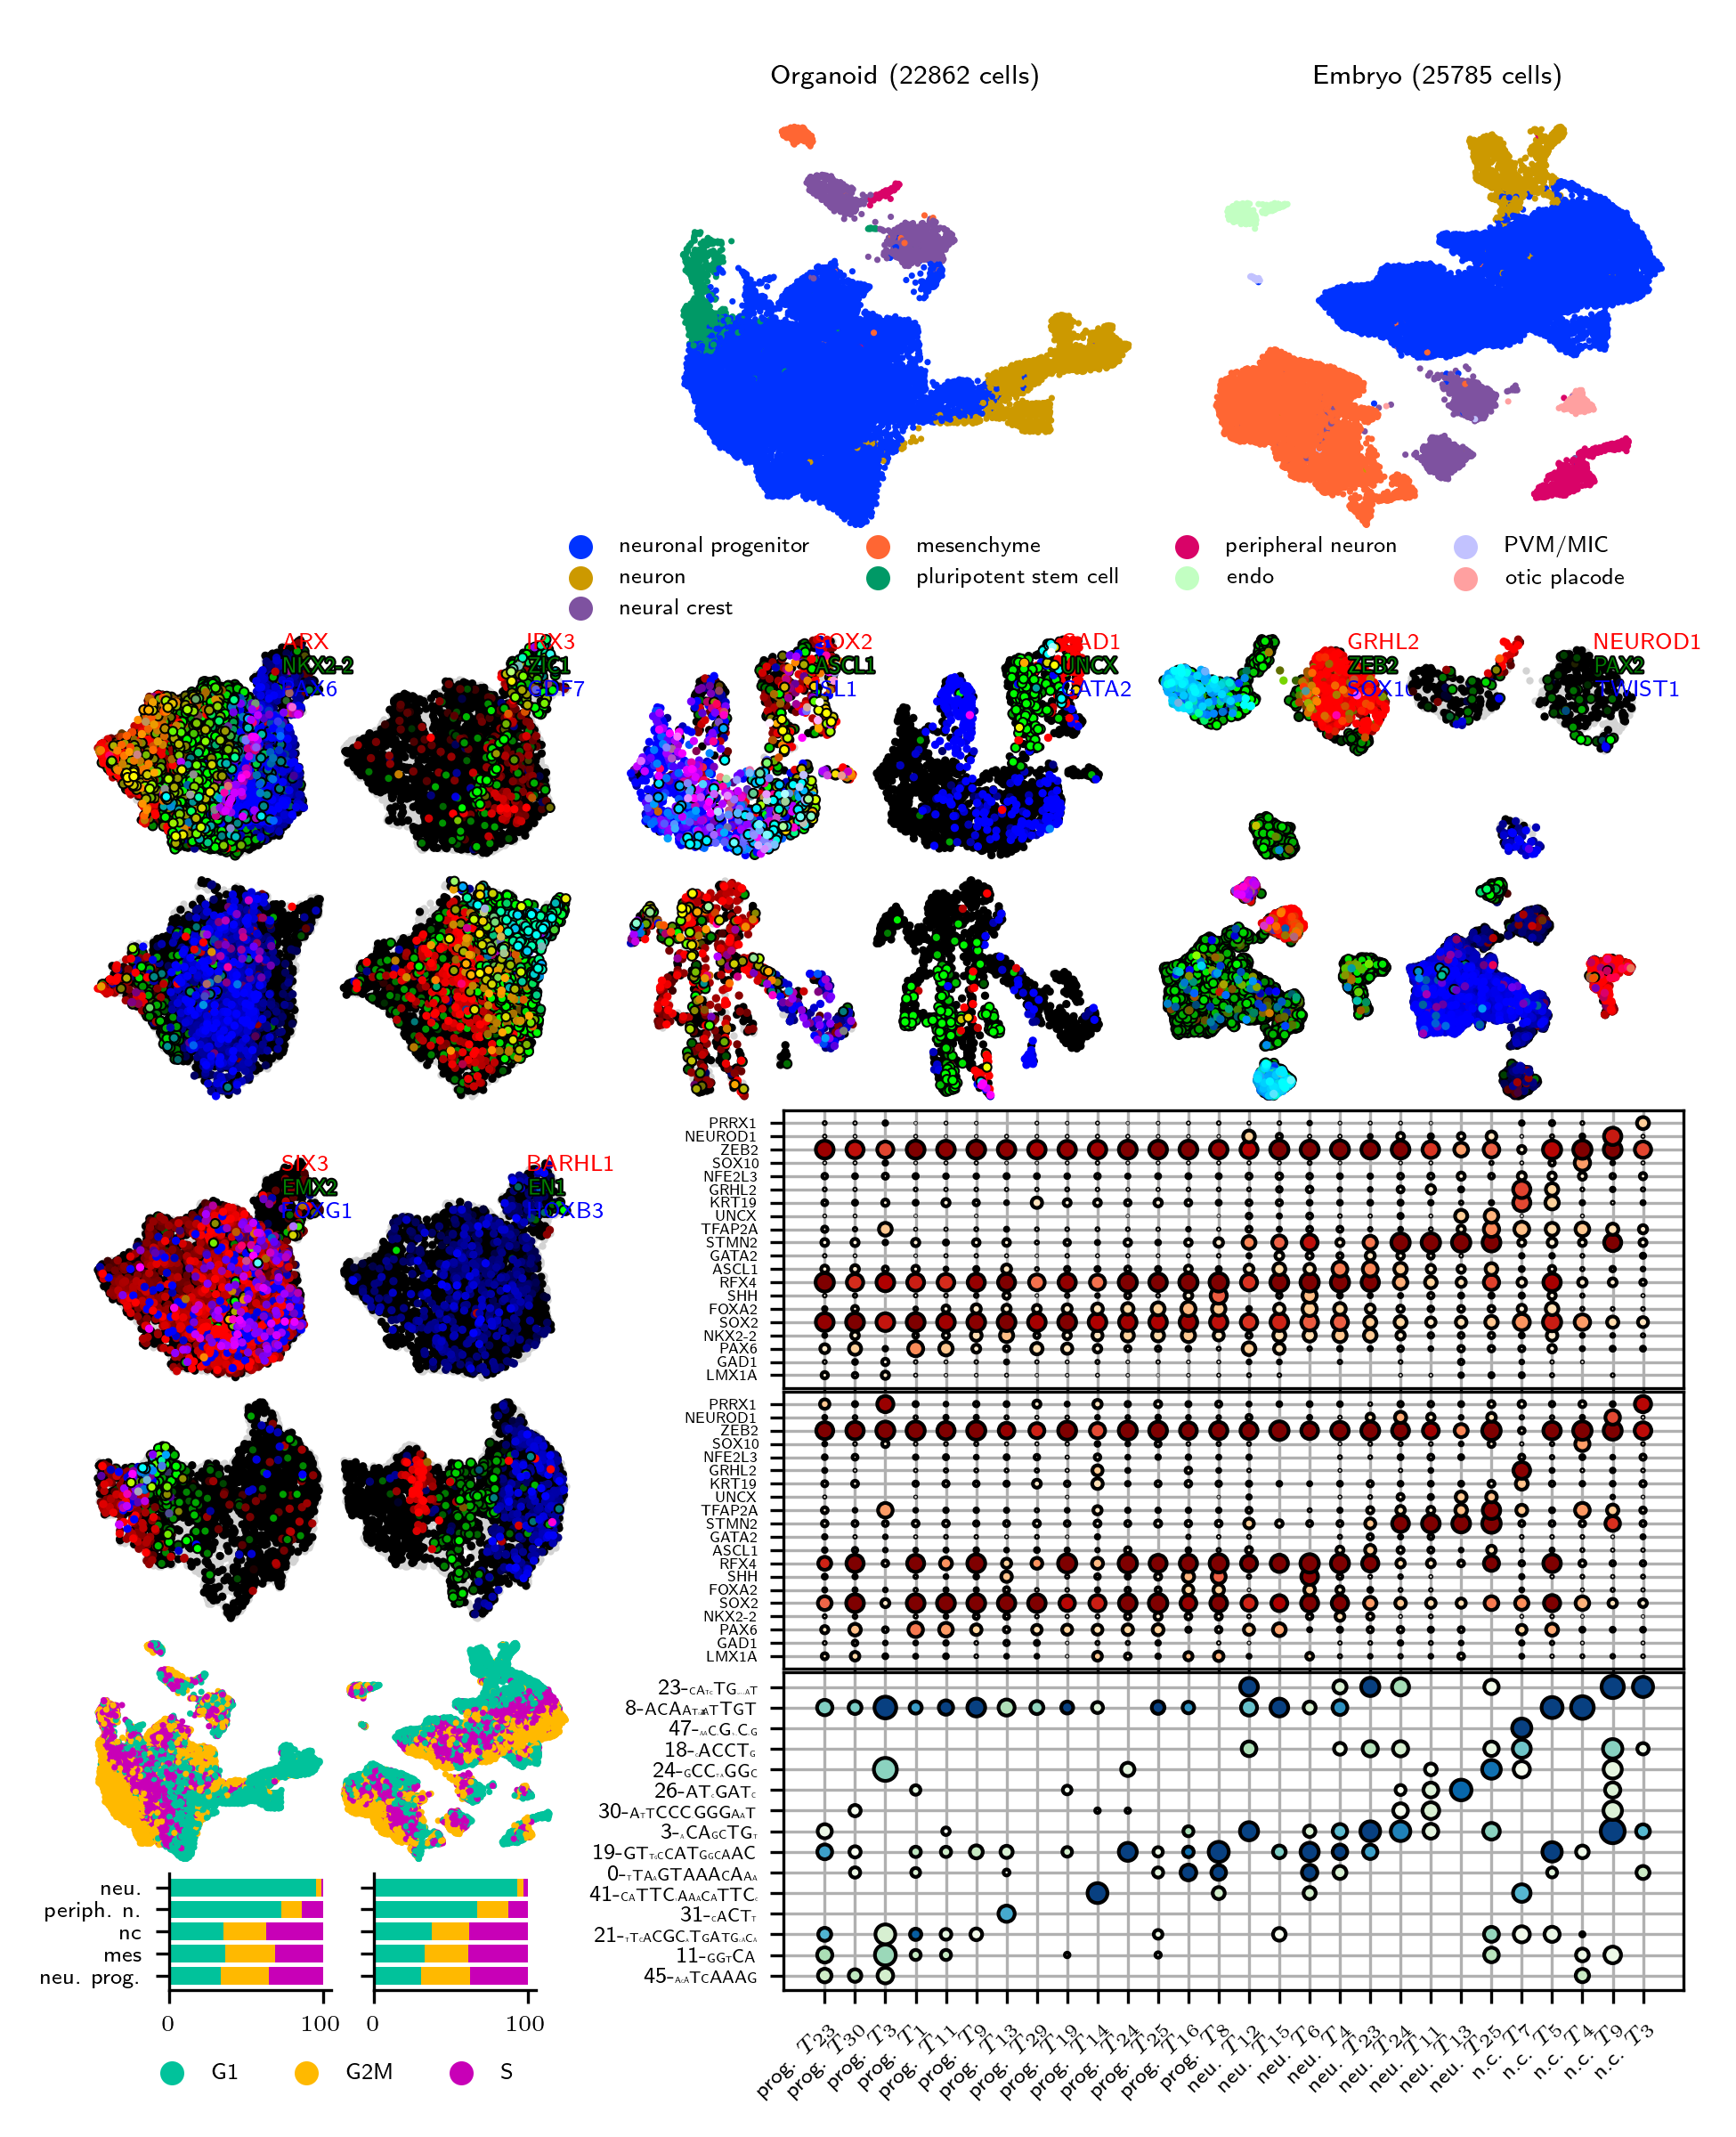
\includegraphics[width=1.0\linewidth]{figures/main/Figure_1.png}

\subsection*{Figure 1. Human neural tube organoids recapitulate early neuronal and neural crest development}

\textbf{a}, Schematic. \textbf{b-c}, UMAP based on gene expression profiles of organoid (\textbf{b}) and embryo
(\textbf{c}) cells colored by cell type identify. \textbf{d-f}, UMAP based on gene expression profiles of organoid (top)
and embryo (bottom) cells types showing sub-clusters of neuronal progenitors (\textbf{d}), early differentiating neurons
(\textbf{e}) and neural crest (\textbf{f}) along with expression of indicated genes in red-green-blue color scale.
\textbf{g}, UMAP based on gene expression profiles of organoid (top; UMAP axis 1 and 2 shown) and embryo (bottom; UMAP
axis 2 and 3 shown) for neuronal progenitor subcluster along with the expression of indicated genes in red-green-blue
color scale. \textbf{h}, UMAP based on gene expression profiles in organoid (top left) and embryo (top right) colored by
cell cycle phase identity and quantification of percentage of each cell for each cell cycle phase stratified by cell
type in the organoid (bottom left) and embryo (bottom right). \textbf{i}, Average gene expression level in
$log_{2}(CPM)$
(dot color) and fraction of cells expressing the gene (dot size) per cell state, defined by topic modeling, for organoid
cells (top) and embryo cells (middle) and motif enrichment level as normalized enrichment score (NES; dot color) and
number of regions enriched for the motif (dot size) per topic (x-axis) and motif (y-axis; bottom). PVM/MIC: perivascular
microphage/microglia.

\subsection*{
  DeepNeuralTube: sequence-to-function models that reveal the enhancer code underlying early neuronal and neural crest 
  development
}

To gain insight into the sequence characteristics underlying cell type-specific activity of neural tube, neural crest
and derived cell type enhancers, we trained two sequence-to-function model convolutional neural networks:
"$DeepNeuralTube_{organoid}$" and "$DeepNeuralTube_{embryo}$". The models use DNA sequence, of genomic regions, as input and
classify the regions based on their cell type- or state-specific chromatin accessibility (in a multi-label multi-class
fashion; \textbf(Fig. 2a)). The classes of the models are defined based on topic modeling. To get a fine-grained
definition of cell states, we performed topic modeling separately for the subset of neuronal progenitors, neural crest
(incl. facial mesenchyme and peripheral neurons) and early differentiating neurons for both the organoid cells (to
train $DeepNeuralTube_{organoid}$) and embryo cells (to train $DeepNeuralTube_{embryo}$). To validate the ability of the models to
predict cell type-specific enhancer \textit{activity}, we tested their performance on enhancers from the VISTA enhancer
browser (\textbf{REF}). Relevant for this study, this database contains enhancers active in the neural tube (n=349) and
facial mesenchyme (n=143). Neural tube enhancers could be classified with an area under the receiver-operator curve
(auROC) of 0.75 and 0.80 using resp. $DeepNeuralTube_{organoid}$ and $DeepNeuralTube_{embryo}$ (\textbf{Fig. 2b}; and
area under the precision-recall curve (auPR) of 0.21 resp. 0.29 (\textbf{FIGURE SUPPLEMENT})), facial mesenchyme
enhancers with an auROC of 0.78 and 0.79 using resp. $DeepNeuralTube_{organoid}$ and $DeepNeuralTube_{embryo}$
(\textbf{Fig. 2c}; and auPR of 0.17 for both models (\textbf{FIGURE SUPPLEMENT})). Of note, a fraction of neural tube
enhancers (x.x \%) are predicted to be specific to pre-migratory neural crest by both models.\par
Next, we wanted to assess the explainability of the models. Concretely we wanted to test whether the model learned known
TF binding motifs as features. For this, we performed motif enrichment analysis on all regions for each topic and
calculated gradients, for each model, on the top 1,000 regions (as predicted by the model) for each topic followed by
TF-MoDISco (\textbf{REF}) to find \textit{de novo} motifs used by the models. For both known motifs and \textit{de novo}
motifs we calculated pairwise similarities using TOMTOM (\textbf{REF}) followed by clustering, resulting in 56 motif
clusters (\textbf{Fig. 2d}). Of note, most clusters contain known-motifs enriched in both organoid regions and embryo
(\textbf{Fig. 2e}) regions with the exception of cluster 13 which is organoid specific (AP1 motif; \textbf{SUPPLEMENTAL TABLE}) and cluster
26 which is embryo specific (CG-rich motif; \textbf{SUPPLEMENTAL TABLE}). Most clusters (\textbf{Fig. 2f-g} and
\textbf{SUPPLEMENTAL FIGURE}) contain at least one motif learned \textit{de novo} by the organoid and/or embryo model.
Thus, $DeepNeuralTube_{organoid}$ and $DeepNeuralTube_{embryo}$ use known-motifs as features to classify regions based
on cell type-specific chromatin accessibility.\par
As an illustrative example, we investigated an enhancer located in one of the introns of GLI3 (hs111.0; \textbf{SUPPLEMENTAL
FIGURE}). This region has neural tube specific activity in E11.5 mouse embryos (\textbf{Fig. 2h}). Both
$DeepNeuralTube_{organoid}$ and $DeepNeuralTube_{embryo}$ explain this region similarly (Pearson correlation of x) and
highlight the importance of multiple SOX TFBS (\textbf{Fig. 2h}). A version of this enhancer where 5\% of the
nucleotides are changed (hs111.1) does not have neural tube specific enhancer activity and both
models predict that this loss of activity is due to the loss of a sinlge SOX TFBS (\textbf{Fig. 2h}).\par
Finally, to also investigate the performance of the models on migratory neural crest, a cell type for which there are no
validated enhancers in the Vista enhancer browser, we selected a genomic region that is specifically accessible in the
migratory neural crest cell type of the organoid (\textbf{SUPPLEMENTAL FIGURE}). Both models predict this region
to be specific to the migratory neural crest class (\textbf{SUPPLEMENTAL FIGURE}) and nucleotide importance scores
reveal TFBS for a SOX monomer, a SOX dimer and AP2 (\textbf{Fig. 2i}). We tested the enhancer activity of this region
using a reporter assay in chicken embryos. Indeed the enhancer was specifically active in migratory neural crest 24
hours after injection in an HH4 embryo (\textbf{Fig. 2i}).\par

\noindent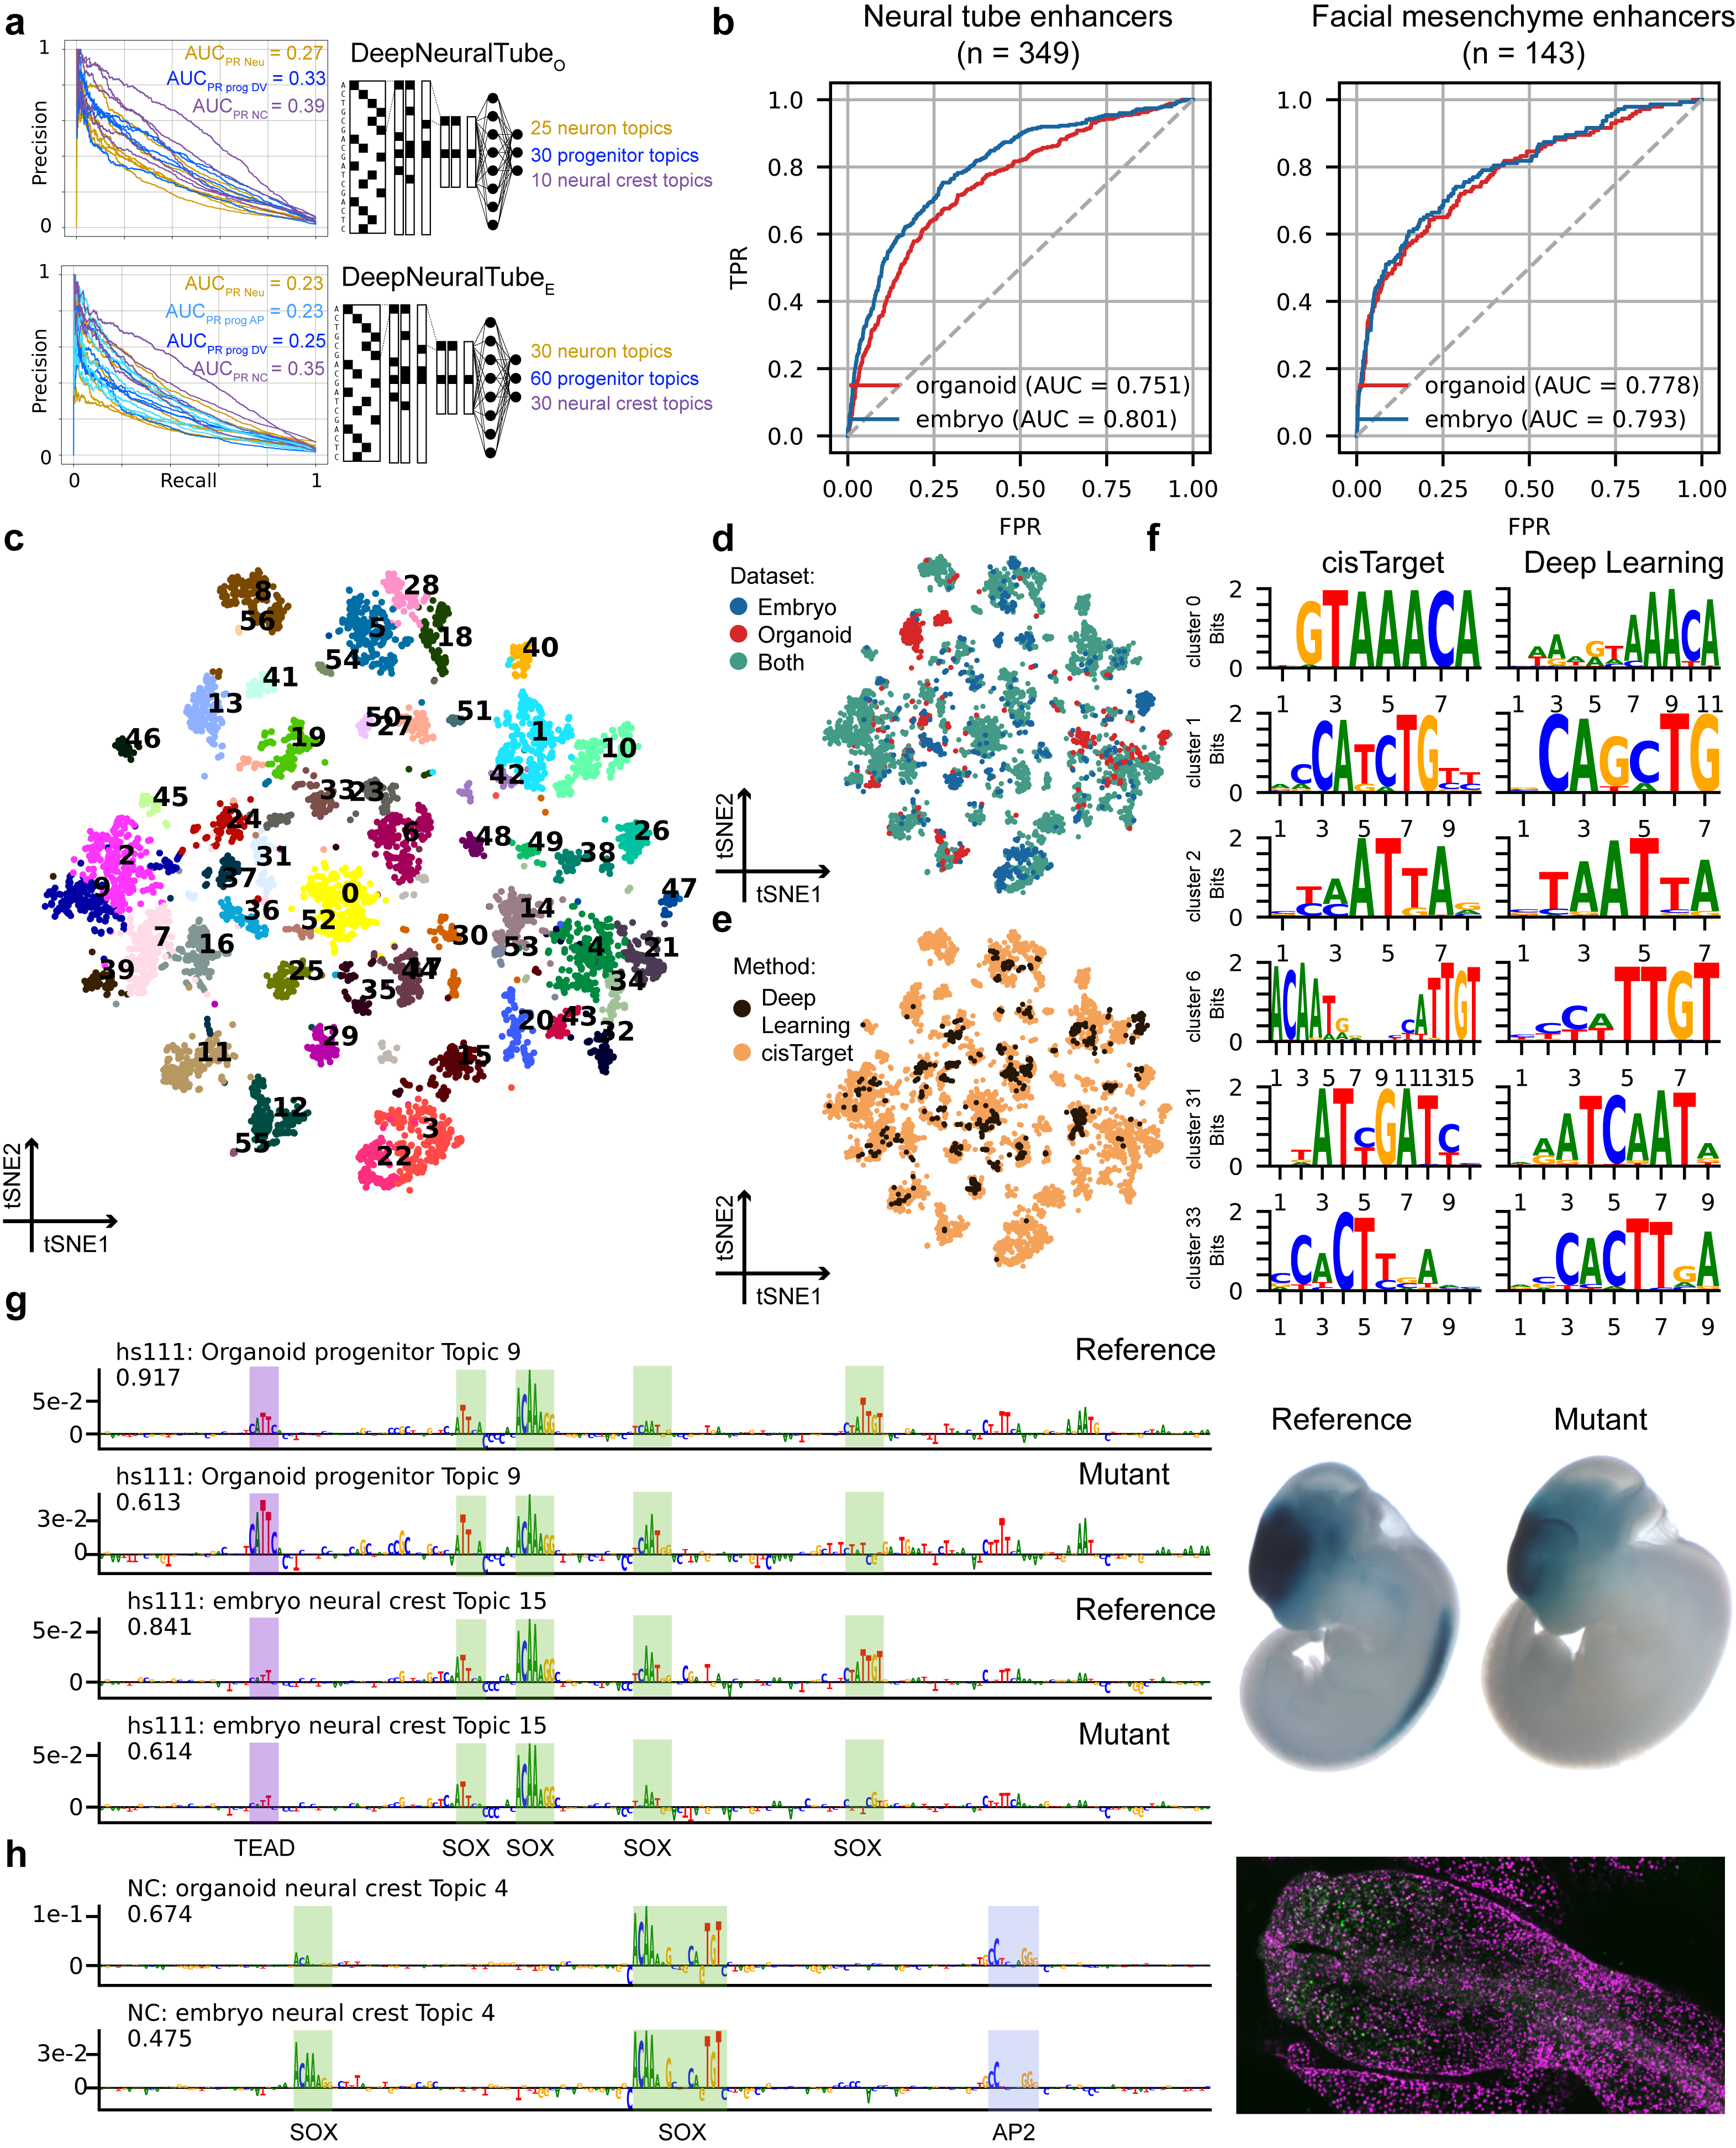
\includegraphics[width=1.0\linewidth]{figures/main/Figure_2.png}

\subsection*{Figure 2. DeepNeuralTube: an accurate sequence-to-function model revealing neuro-developmental enhancer
code.}
\textbf{a}, Schematic. \textbf{b} receiver-operator curves for identifying neural tube (left) and facial mesenchyme the
$DeepNeuralTube_{organoid}$ and $DeepNeuralTube_{embryo}$. \textbf{c-e}, UMAP of TomTom [REF] motif-to-motif similarities
using both \textit{de novo} motifs from DeepNeuralTube and known enriched motifs. Each dot is a motif. Motifs are
colored by: cluster identity (\textbf{c}), model of origin (\textbf{d}; only showing \textit{de novo} motifs in this
case) and whether the motif is found \textit{de novo} (Deep Learning) or by motif enrichment (cisTarget; \textbf{e}).
\textbf{f}, Example representative motifs from clusters in b, showing motifs from motif enrichment (left) and found
\textit{de novo} (right). \textbf{g}, contribution score for reference and mutant version of Vista enhancer hs111
for $DeepNeuralTube_{organoid}$ (top two panels) and $DeepNeuralTube_{embryo}$ (bottom two panels) and enhancer-reporter
assay for reference and mutant version of hs111 (right two panels) [REF]. \textbf{h}, contribution score for
$DeepNeuralTube_{organoid}$ (top) and $DeepNeuralTube_{embryo}$ (bottom) of a genomic enhancer human neural crest
enhancer (chr ...; hg38) and enhancer-reporter assay in chicken embryo (HH4; right). Green is enhancer signal, pink is
constitutive enhancer that serves as electroporation control.

\subsection*{
  Deciphering the enhancer code underlying dorso-ventral patterning of neuronal progenitors
}
Focusing on neuronal progenitors, we identified topics representing cells and regions of different dorso-ventral
identities in both the organoid and the embryo data (\textbf{Fig. 3a}). From ventral to dorsal this is topic 36, 38, 33,
54 and 48 in the organoid data and topic 34, 38, 79, 88 and 58 in the embryo data. As an example we first investigated
two enhancers of \textit{SHH} that are strongly conserved and specific to the floorplate [\textbf{REF}]; SFPE1 and SFPE2.
\textit{SHH} is most strongly expressed in the most ventral topic (33 and 34 resp. in the organoids and the embryo; \textbf{Fig. 3b}).
SFPE1 is located upstream of \textit{SHH} and SFPE2 in its second intron. Both enhancers are indeed most accessible in the cells
belonging to the ventral topic, in both the organoid and embryo data (\textbf{Fig. 3c}). Explaining the accessibility of both
enhancers using DeepNeuralTube reveals two FOX (one partial), one SOX and two RFX (one partial) binding sites in SFPE1
and two FOX and a TEAD binding site in SFPE2 (\textbf{Fig. 3d}).\par

To investigate the enhancer code underlying dorso-ventral patterning of neuronal progenitors further, we calculated
contribution scores on the top 1,000 regions of each organoid and embryo dorso-ventral topic using respectively $DeepNeuralTube_{organoid}$ and $DeepNeuralTube_{embryo}$. We then used TF-MoDISco\cite{shrikumar2020tfmodisco} to find reoccurring seqlets for each topic (patterns) and we clustered patterns based on pairwise motif similarities (SUPPLEMENTAL FIG). Next, we calculated the average contribution for all identified instances per cluster and for each topic resulting in a dorso-ventral enhancer code table (\textbf{Fig. 3e}). Both $DeepNeuralTube_{organoid}$ and $DeepNeuralTube_{embryo}$ found similar patterns
underlying the different dorso-ventral states and the importance of the instances of these patterns is highly correlated across both
models (CORR COEF; \textbf{Fig. 3e}). For the most ventral state (organoid topic 33 and embryo topic 34) a combination of FOX, TEAD
and RFX instances is important (\textbf{Fig. 3e-f}) and the importance of these instances correlates with the expression of respectively \textit{FOXA2}, \textit{TEAD1} and \textit{RFX4} in both the organoid and embryo cells (\textbf{Fig. 3g}). In subsequent more dorsal neuronal progenitor domains we observe importance of NKX instances, correlating with \textit{NKX2-2} expression (\textbf{(Fig. 3e- g)}); PAX instances, correlating with \textit{PAX6} expression (\textbf{Fig. 3e-g}) and ZIC instances, correlating with \textit{ZIC1} expression (\textbf{Fig. 3e-g}). For all dorso-ventral progenitor domains, except the most ventral one (and the most dorsal one in the embryo), SOX instances are important which correlates with \textit{SOX2} expression. Similarly, ZEB instances have a negative importance to the accessibility of regions in dorso-ventral domains except the most ventral one (\textbf{Fig. 3e}). Finally, we calculated the Jaccard index of genomic regions based on the presence of an instance of each identified pattern to investigate which patterns often co-occur in the same regions (\textbf{Fig. 3h}). FOXA2, TEAD1 and RFX4 instances often co-occur in the same genomic region while instances of other patterns seem to be present in separate regions (\textbf{Fig. 3h}).\par

It has been reported that FOXA2 is a pioneer factor. Indeed, when centering on FOXA2 instances in both the organoid and
embryo data we observe a strong footprint when looking at Tn5 cut-sites (\textbf{Fig. 3i} and SUPPLEMENTAL FIG). We then
asked if there is any difference between regions that are generally bound by FOXA2 in any cell state that expresses this
TF and regions, bound by FOXA2, that are specific to the floorplate. For this purpose, we downloaded FOXA2 ChIP-seq
peaks in HepG2 and A549 and intersected these with floorplate peaks containing FOXA2 instances. Those floorplate peaks
that overlapped with both ChIP-seq datasets we classified as regions that are generally bound by FOXA2 and those that
did not we classified as floorplate specific. Next, we quantified both the number of FOXA2 instances per region and the
affinity of each individual instance (making use of the FOXA2 motif score calculated using
FIMO\cite{grant2011fimo,schreiber2025tangermeme}) hypothesizing that the overall affinity of regions that are generally
bound by FOXA2 is higher than floorplate specific regions either because these general regions have more instances or
the affinity of individual instances is higher. Indeed, FOXA2 target regions that are specific to the floorplate mostly
have a single FOXA2 instance while FOXA2 target regions that are general tend to have more instances (\textbf{Fig. 3j}).
Furthermore, in case there is but a single FOXA2 instance in a general FOXA2 target the affinity of this instance tends
to be higher (\textbf{Fig. 3k}). Generating a \textit{de novo} motif from general and specific FOXA2 target regions that
have a single instance, we observe that FOXA2 instances in regions that are general tend to be of the form
\textit{TGTTT\underline{AC}} while those instances in specific regions tend to be of the form \textit{TGTTT} (\textbf{Fig. 3l}).\par


\noindent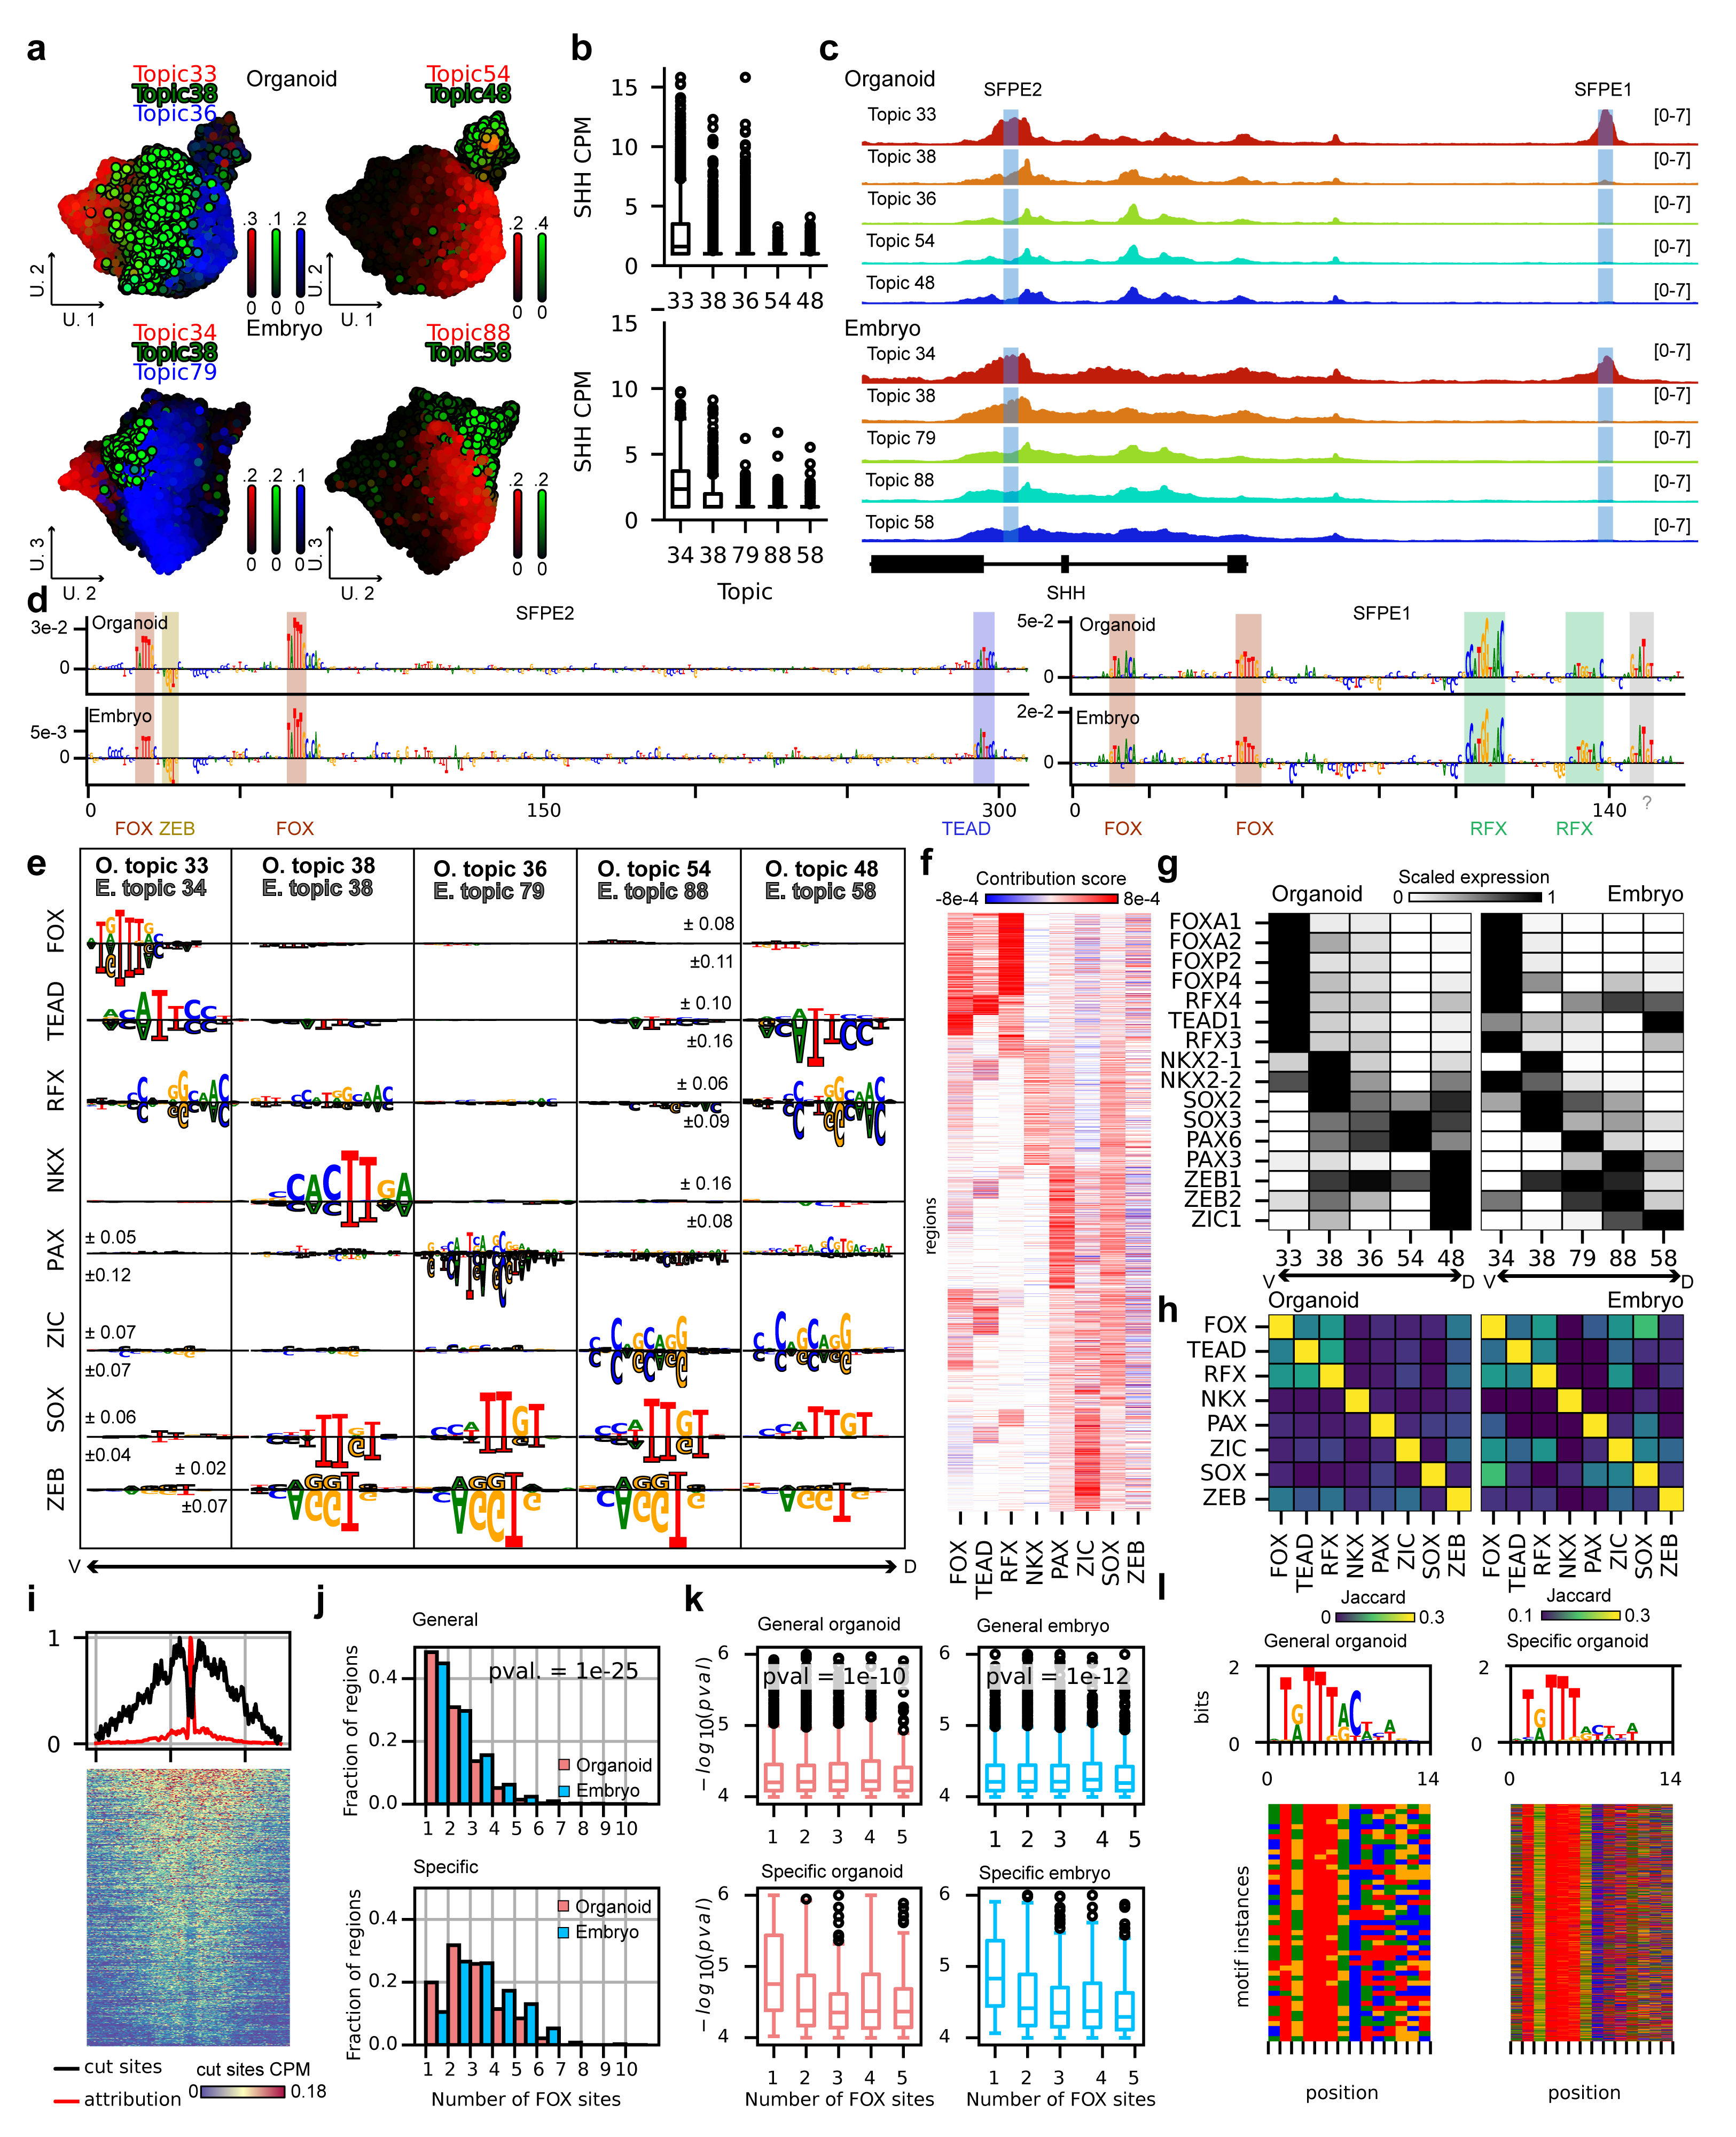
\includegraphics[width=1.0\linewidth]{figures/main/Figure_3.png}

\subsection*{
  Figure 3. Deciphering the enhancer code underlying dorso-ventral patterning of neuronal progenitors.
}
\textbf{a}, UMAP of organoid (top) and embryo (bottom) neuronal progenitors colored by cell-topic probabilities in RGB color scales of dorso-ventral topics. \textbf{b}, Boxplots of the expression of \textit{SHH} in organoid (top) and embryo (bottom) across different dorso-ventral topics ($n_{topic 33}$ = X, $n_{topic 38}$ = X, $n_{topic 36}$ = X, $n_{topic 54}$ = , and $n_{topic 48}$ = for organoid cells; and $n_{topic 34}$ = X, $n_{topic 38}$ = X, $n_{topic 79}$ = X, $n_{topic 88}$ = , and $n_{topic 58}$ = for embryo cells). \textbf{c}, Chromatin accessibility in organoid (top) and embryo (bottom) across dorso-ventral topics for locus chr:...-...; hg38. SFPE2 and SFPE1 is highlighted. \textbf{d}, Nucleotide contribution scores for SFPE2 (left) and SFPE1 (right) for organoid topic 33 (top) and embryo topic 34 (bottom). \textbf{e}, Code table showing average contribution score of pattern instances for each dorso-ventral topic. Contribution scores for $DeepNeuralTube_{organoid}$ are not outlined. Contribution scores for $DeepNeuralTube_{embryo}$ are outlined and negated. \textbf{f}, Heatmap showing the maximum normalized contribution score for each of the top 1,000 regions per topic (y-axis) and pattern (x-axis) for dorso-ventral topics. \textbf{g}, Heatmap showing scaled expression of transcription factors corresponding to identified patterns in organoid (left) and embryo (right) dorso-ventral topics. \textbf{h}, Heatmap showing Jaccard index of regions based on the presence of instances of the identified patterns. \textbf{i}, Scaled average and normalized number of cut sites (black, top) and contribution score (red, top) across genomic regions with a FOXA2 instance and heatmap showing normalized number of cut sites (bottom) for individual regions with a FOXA2 instance. Signal is centered on the FOXA2 instance start position. \textbf{j}, Bar chart showing the fraction of genomic regions that has a given number of FOXA2 instances for FOXA2 regions that overlap with HepG2 or A549 FOXA2 ChIp-seq signal (general; bottom) and those regions that don't overlap (specific; top). \textbf{k}, Boxplot (ADD NUMEBRS) showing $-log_10(p value)$ of FOXA2 motif hits calculated using FIMO\cite{grant2011fimo,schreiber2025tangermeme} for general regions (bottom) and specific regions (top) stratified by the number of FOXA2 instance per region. \textbf{l}, \textit{de novo} motif for regions with a single FOXA2 instance that are specific (left, top) or general (right, top) and heatmap color coded by nucleotide identity for individual regions for both specific (left, bottom) and general (right, bottom) regions that have a single FOXA2 instance. 

\subsection*{
  Anterior-posterior patterning in neuronal progenitors is regulated by different homeodomain transcription factors that
  each recognize a distinct binding site.
}

Given that we observed cell states from different AP domains in the neuronal progenitors from the embryo (but not
organoid; see \textbf{Fig. 1}) we decided to study the gene regulatory code underlying this patterning further. We
identified seven topics corresponding to different AP domains, from anterior to posterior this is Topic 61, Topic 59,
Topic 31, Topic 62, Topic 70, Topic 52 and Topic 71 (\textbf{Fig. 4a}). We first asked if the AP-program is distinct
from the DV program. In other words, is AP patterning encoded in the same or in different genomic regions as in those in
which DV patterning is encoded? For this purpose, we calculated the pairwise correlation between region-topic
probabilities of all AP and DV topics (\textbf{Fig. 4b}). From this it is clear that both AP and DV patterning as well
as each of their sub-domains are mostly encoded in distinct genomic regions, with the exception of AP Topic 59 and 31
that correlate with the region-topic probability of DV Topic 38 (which corresponds to cells expressing \textit{NKX2-2}; \textbf{Fig. 4b})\par

$DeepNeuralTube_{embryo}$ was able to distinguish the different AP domains but grouped topics of similar domains
together (i.e., Topic 59, 31 and 62; Topic 52 and 71), resulting in four distinct AP domains (\textbf{Fig.4 c-d}). By
explaining the predictions of $DeepNeuralTube_{embryo}$ on the regions of those domains we found four distinct
homeodomain TF binding motifs, one for each domain (\textbf{Fig. 4e}). From anterior to posterior this is \textit{TAATTA}, \textit{GGATTA}, \textit{TCATGWTGANTGA} and \textit{CATYMATCA} corresponding with the expression of respectively \textit{SIX3}, \textit{EMX2}, \textit{FOXG1}, \textit{BARHL1}, \textit{EN1} and \textit{HOXB3} [ADD GENE EXPRESSION HEATMAP!]. Finally, SOX2 instances are present in regions of all AP domains (\textbf{Fig. 4e}).\par

Focusing on the two most anterior domains, two similar homeodomain TF binding motifs seem to underlie the differential
accessibility of those domains. Both have the core homeobox motif: \textit{TAAT} but one is flanked by the nucleotides \textit{TAG} while the other is flanked by the nucleotides \textit{CCCT}. We were surprised that this slight difference in the two motifs would be enough for encoding two separate AP domains. To test this hypothesis, we first did a substitution experiment where we replaced all instances of \textit{CTAAT\underline{TAG}} with \textit{CTAAT\underline{CCCT}} in regions of the most anterior domain and vice versa (\textbf{Fig. 4f}). Indeed, $DeepNeuralTube_{embryo}$ predicts an anterior-to-posterior shift of accessibility of those regions after the \textit{CTAAT\underline{TAG}} to \textit{CTAAT\underline{CCCT}} substitution and vice versa a posterior-to-anterior shift of accessibility after the \textit{CTAAT\underline{TAG}} with \textit{CTAAT\underline{CCCT}} to  \textit{CTAAT\underline{TAG}} substitution (\textbf{Fig. 4f}). Next, we designed enhancers from scratch by embedding either the  \textit{CTAAT\underline{TAG}} or \textit{CTAAT\underline{CCCT}} motif\cite{taskiran2024synthetic, kempynck2025crested} and using respectively Topic 61 and Topic 31 as target class (\textbf{Fig. 4g}). [SWITCH PANELS]. Embedding of two instances of either motif was sufficient to reach predicted chromatin accessibility levels of equivalent ranges to the predicted chromatin accessibility levels of genomic regions (\textbf{Fig. 4g}). Next, to eliminate potential model bias we repeated the same experiment but optimized for the opposite class. This is, we optimized for Topic 31 by embedding the \textit{CTAAT\underline{TAG}} motif optimized for Topic 61 by embedding the \textit{CTAAT\underline{CCCT}} motif (\textbf{Fig. 4h}). In this case, the synthetic design failed to converge for the target class but instead regions with high prediction score for the AP domain that corresponds to the motif used for embedding were generated. This is embedding of the \textit{CTAAT\underline{TAG}} motif still generated regions with high prediction score for Topic 61 and embedding of the \textit{CTAAT\underline{CCCT}} motif generated regions with high prediction score for Topic 31 (\textbf{Fig. 4h}).\par

From these results it seems that a relatively simplistic code using two distinct motifs is sufficient to distinguish between the two utmost neuronal progenitor AP domains. Encouraged by this finding, we trained a logistic regression model to classify genomic regions of those two domains in either Topic 61 or Topic 31 using as features only the motif scores of the two motifs identified above (\textbf{Fig. 4i}). Surprisingly, this very simple classifier reached high performance with area under the ROC of X and area under the precision recall curve of X (\textbf{Fig. 4i}).\par


\noindent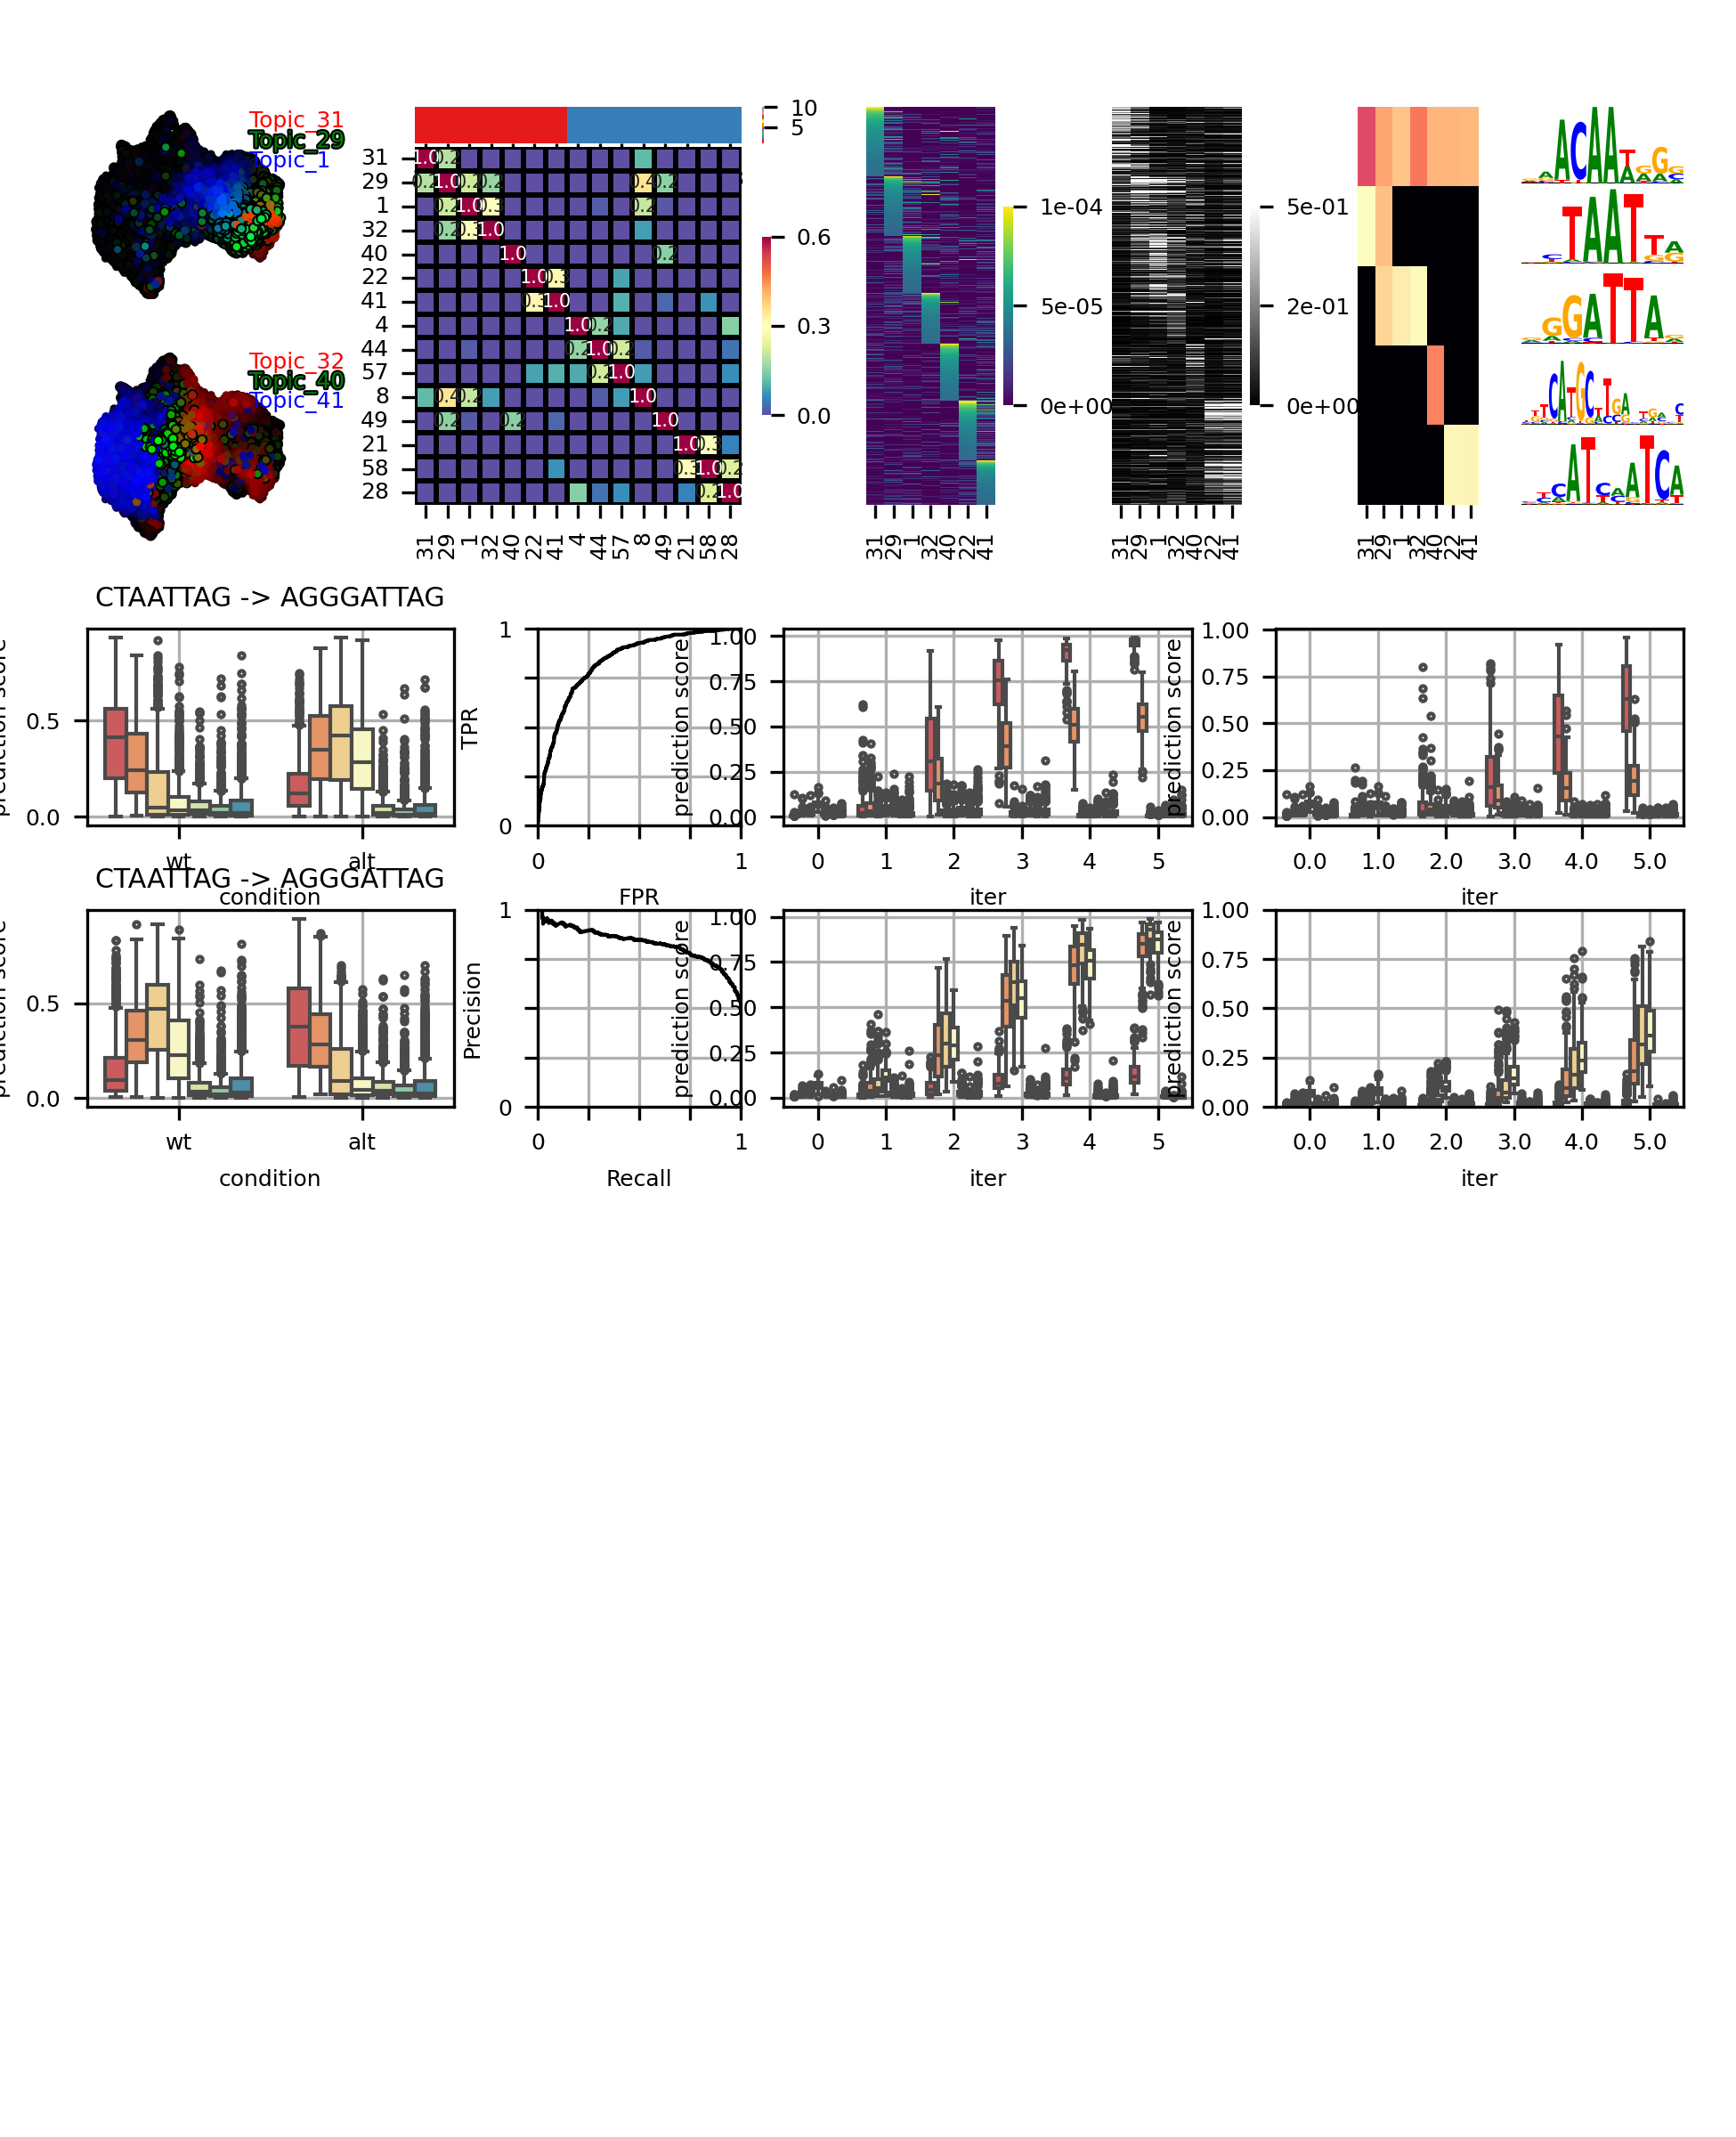
\includegraphics[width=1.0\linewidth]{figures/main/Figure_4.png}

\subsection*{
Figure 4. A simple enhancer code underlies anterior-posterior patterning in neuronal progenitors.
}
\textbf{a}, UMAP of embryo neuronal progenitors colored by cell-topic probabilities in RGB color scales for
anterior-posterior topics. \textbf{b}, Heatmap showing pairwise pearson correlation coefficients of region-topic probabilities for dorso-ventral and anterior-posterior topics. \textbf{c}, Heatmap showing region-topic probabilities for the top 3,000 regions per topic (y-axis) and each anterior-posterior topic (x-axis). \textbf{d}, Heatmap showing prediction scores of $DeepNeuralTube_{embryo}$ on the topic 3,000 regions per topic (y-axis) for each anterior-posterior topics (x-axis).\textbf{e}, Heatmap showing the log of the number of seqlets for each identified pattern (y-axis) for all anterior-posterior topics (x-axis).\textbf{f}, Boxplot showing prediction score before (wt) and after (alt) substituting all instances of \textit{CTAATTAG} with \textit{CTAATCCCT} (top) or substituting all instances of \textit{CTAATCCCT} with \textit{CTAATTAG} (bottom) in the topic 3,000 regions of either Topic 61 or Topic 31. \textbf{g}, Boxplot showing prediction scores for all anterior-posterior topics after embedding 0 to 5 instances of \textit{CTAATTAG} while optimizing their location for Topic 61 (top) and after embedding 0 to 5 instances of \textit{CTAATCCCT} while optimzing their location for Topic 31 (bottom); n = 200. \textbf{h}, Boxplot showing prediction scores for all anterior-posterior topics after embedding 0 to 5 instances of \textit{CTAATTAG} while optimizing their location for Topic 31 (top) and after embedding 0 to 5 instances of \textit{CTAATCCCT} while optimzing their location for Topic 61 (bottom); n = 200. .\textbf{i}, receiver-operator curve (ROC) (top) and precision-recall curve (bottom) for logistic regression classifier classifying genomic regions as either Topic 61 or Topic 31 based on motif scores for \textit{CTAATTAG} and \textit{CTAATCCCT} motifs.

\subsection*{
  Deciphering the enhancer code underlying pre-migratory and migratory neural crest and facial mesenchyme.
}

Focusing on neural crest cells, we identified topics representing cells and regions of both pre- and migratory neural
crest as well as facial mesenchyme (\textbf{Fig. 5a}). Similar to the neuronal progenitors, we used
$DeepNeuralTube_{oranoid}$ and $DeepNeuralTube_{embryo}$ to explain the top 1,000 regions for each organoid and embryo
topic and generated a code table based on the identified pattern instances (\textbf{Fig. 5b}). Again, both
$DeepNeuralTube_{organoid}$ and $DeepNeuralTube_{embryo}$ found similar patterns and the importance of the instances fo
these patterns is highly correlated across both models (CORR COEF; \textbf{Fig. 5b}).\par

Organoid Topic 62 and embryo Topic 103 represent the pre-migratory neural crest state and instances of TEAD, GRHL, AP2 and ZEB patterns are important for this state (\textbf{Fig. 5b-c}) the importance of TEAD instances correlates with \textit{TEAD4} expression, GRHL with both \textit{GRHL1} and \textit{GRHL2} and AP2 with both \textit{TFAP2A} and \textit{TFAP2C} (\textbf{Fig. 5d}). Note that ZEB instances have a positive contribution to the pre-migratory while it has a negative contribution to all other neural crest states (\textbf{Fig. 5b-c}) and moreover all other states of both the neuronal progenitors (\textbf{Fig. 3e}) and neurons (\textbf{Fig. 6b}). The positive contribution of ZEB in the pre-migratory neural crest state coincides with the absence of the expression of both \textit{ZEB1} and \textit{ZEB2} (\textbf{Fig. 5d}). This is in line with the previously reported role of ZEB2 as a chromatin closing repressor \cite{taskiran2024synthetic}.\par

The migratory neural crest cell state is represented by two organoid topics (Topic 65 and 59) and a single embryo topic (Topic 94). Nuclear receptor, AP2, ZIC (only in organoid topics) and SOX-dimer (organoid Topic 59 but not 65) are important for this state (\textbf{Fig. 5b-c}). We could not link the nuclear receptor instances to a specific TF based on the correlation of expression and the importance score of these instances. The importance of AP2 instances correlates with the expression of \textit{TFAP2A}, \textit{TFAP2B} and \textit{TFAP2C} (\textbf{Fig. 5d}), ZIC with \textit{ZIC1} to \textit{ZIC5} and the SOX-dimer with expression of \textit{SOX10}. The switch from TFAP2A/C in pre-migratory neural crest to TFAP2A/B in migratory neural crest is consistent with a previously reported function of both heterodimers in respectively neural plate border induction and neural crest specification\cite{rothstein2020heterodmerization}. After the pre-migratory and before the migratory neural crest state another topic is found in both organoid (Topic 60) and embryo (Topic 105) for which instances of RFX are important (\textbf{Fig. 5b-c}) that correlate with the expression of \textit{RFX4} (\textbf{Fig. 5d}).\par

Finally, the facial mesenchyme cell state is represented by organoid Topic 58 and embryo Topic 91. Instances of a FOX
pattern and a dimer consisting of a homeobox and ebox motif are important for this state (\textbf{Fig. 5b}). The
importance of the FOX instances correlates with the expression of \textit{FOXC2} and that of the dimer motif with the
expression of both \textit{TWIST1} and \textit{ALX4}. The latter is consistent with a recent study where it has been
shown that TWIST1 and ALX4 cooperatively bind this specific dimer motif regulating the expression of genes involved in
facial mesenchyme\cite{kim2024dnaguided}.\par

Next, we investigated which patterns co-occur in the same genomic regions. For this purpose, we calculated the Jaccard
index of genomic regions based on the presence of an instance of each identified pattern (\textbf{Fig. 5e}). Using this
method we found three sets of regions that are predicted to be contain instances of different TFs. One set where
instances of TEAD4, GRHL1/2 and ZEB1/2 co-occur, one where instances of Nuclear receptor, TFAP2A/B/C and ZIC1-5
instances co-occur and one set where instances of FOXC2 and TWIST1/ALX4 co-occur.\par

Recently, a genome wide association study (GWAS) was published identifying 203 single-nucleotide polymorphisms (SNPs)
that are associated with facial variation\cite{white2021insights}. Given that regions surrounding these SNPs were
enriched for enhancer activity in cranial neural crest cells\cite{white2021insights} we asked if, using
$DeepNeuralTube$, we could explain the effect of some of these variants on enhancer activity. Therefore for all
suggestive SNPs we scored both the reference and alternative allele(s) using both $DeepNeuralTube_{organoid}$ and $DeepNeuralTube_{embryo}$ and calculated the difference in prediction score across both alleles (delta prediction score). At an absolute delta prediction score threshold of 0.5 we identified X SNPs that we deem explainable by either of the two models. Note that only very few (X out of 203) of these "explainable" SNPs overlap with the 203 lead SNPs identified by White \textit{et al.} (\textbf{Fig. 5f}). Most of the "explainable" SNPs have a high delta prediction score for either organoid neural crest Topic 58 or Topic 59 (SUPPLEMENTAL FIG). As an example we show the explanation of rs1555067 which is located upstream of \textit{PRRX1}. The G>A substitution of this SNP causes a delta prediction score of 0.X for organoid Topic 58 (\textbf{Fig. 5g}), increasing the predicted chromatin accessibility of this genomic region in the facial mesenchyme cell state. This predicted increase in chromatin accessibility is caused by generating an EBOX site 6bp upsteam of a partial homeobox site potentially creating a new binding site for TWIST1-ALX4 dimers (\textbf{Fig. 5h}).\par

\noindent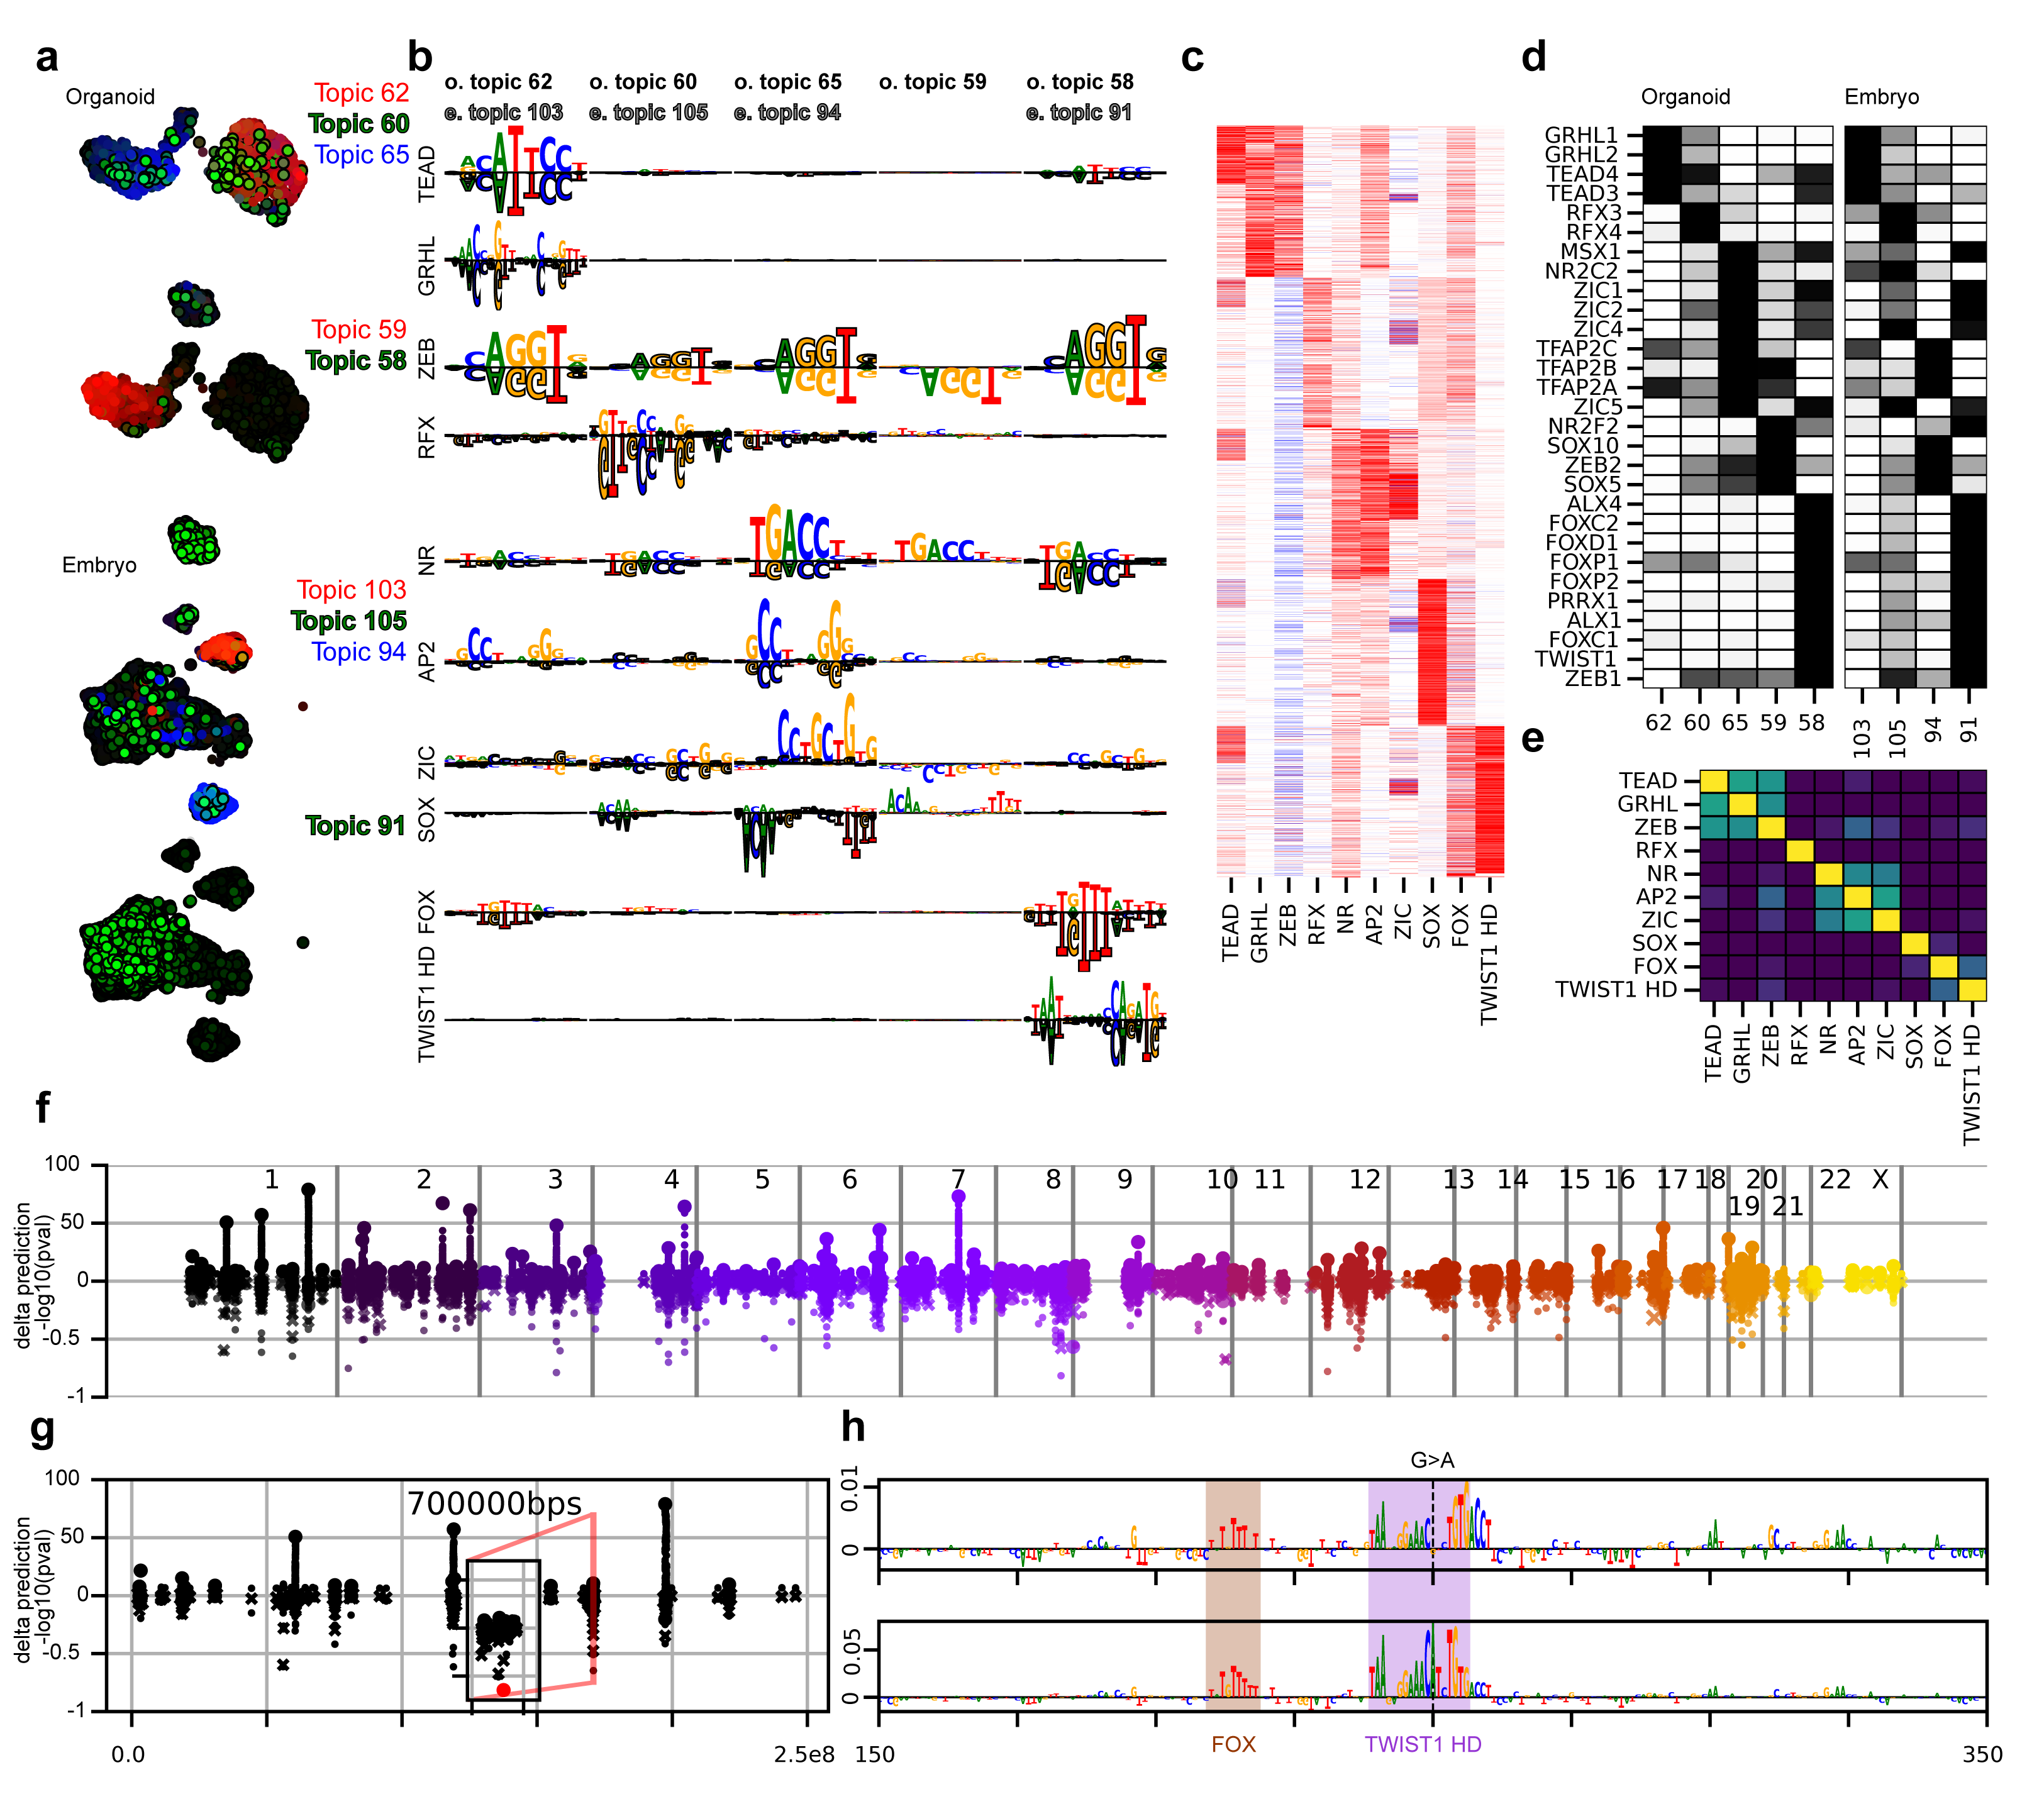
\includegraphics[width=1.0\linewidth]{figures/main/Figure_5.png}

\subsection*{
  Figure 5. Deciphering the enhancer code underlying pre-migratory and migratory neural crest and facial mesenchyme.
}
\textbf{a}, UMAP of organoid (top two) and embryo (bottom two) neural crest cells colored by cell-topic probabilities in RGB color scales for neural crest related topics. \textbf{b}, Code table showing average contribution score of pattern instances for each neural crest related topic. Contribution scores for $DeepNeuralTube_{organoid}$ are not outlined. Contribution scores for $DeepNeuralTube_{embryo}$ are outlined and negated. \textbf{c}, Heatmap showing the maximum normalized contribution score for each of the top 1,000 regions per topic (y-axis) and pattern (x-axis) of neural crest related topics. \textbf{d}, Heatmap showing scaled expression of transcription factors corresponding to identified patterns in organoid (left) and embryo (right) for neural crest related topics. \textbf{e}, Heatmap showing Jaccard index of regions based on the presence of instances of the identified patterns. \textbf{f}, Manhattan plot showing -log p value of the SNP being associated with variations in facial shape\cite{white2021insights} (positive y-axis) and the maximum (across classes of the model) of the absolute value of the difference in prediction score between the reference and alternative allele (negative y-axis; circles for $DeepNeuralTube_{organoid}$ and crosses for $DeepNeuralTube_{embryo}$) across the human genome. Lead SNPs are shown with a bigger dot size. \textbf{g}, Zoom in of chromosome one with the locus of SNP rs1555067 shown as an inset, the SNP itself is shown in red. \textbf{h}, Nucleotide contribution scores for Topic 58 of $DeepNeuralTube_{organoid}$ of the references (top) and alternative (bottom) allele of SNP rs1555067. The location of the SNP is indicated with a dotted line.

\subsection*{
  Deciphering the enhancer code underlying early neuronal differentiation.
}

Focusing on early neuronal differentiation, we identified several topics for different stages of neuronal fate
acquisition in both organoid and embryo cells (\textbf{Fig. 6a}). Again we made use of $DeepNeuralTube_{organoid}$ and
$DeepNeuralTube_{embryo}$ to explain the top 1,000 regions for each topic and generated a code table based on the
identified pattern instances (\textbf{Fig. 6b}). Both models found similar patterns and the importance of the instances
of these patterns is highly correlated across both models (CORR COEF; \textbf{Fig. 6b}).\par

For both the organoid and embryo we found two topics (organoid Topic 6 and 4 and embryo Topic 10 and 18) for which
instances of patterns from neuronal progenitors, more precisely the floorplate, are important (\textbf{Fig. 6b-c}).
These include instances of TEAD, FOX and RFX (\textbf{Fig. 6b-c}) correlating with the expression of respectively \textit{TEAD4/1},
\textit{FOXA2} and \textit{RFX4} (\textbf{Fig. 6d}). Instances of a SOX monomer motif is important for one of these topics (\textbf{Fig. 6b-c}), correlating with the expression of \textit{SOX2} (\textbf{Fig. 6d}). Next, in both organoids and embryo cells we identified a topic for which both instances of neuronal progenitor patterns as well as an EBOX pattern is important (organoid Topic 23 and embryo Topic 13 \textbf{Fig. 6b-c}) the importance of this EBOX pattern correlates with the expression of \textit{ASCL1}. For subsequent topics SOX2 instances are not important anymore (\textbf{Fig. 6b-c}) and we find topics with a where a combination of EBOX and EBF instances are important (organoid and embryo Topic 24\textbf{Fig. 6b-c}) the latter correlating with the expression of \textit{EBF1-3} (\textbf{Fig. 6d}) and topics where a combination of EBF and ONECUT instances are important (organoid Topic 13 and embryo Topic 18; \textbf{Fig. 6b-c}), the latter correlating with the expression of \textit{ONECUT1-3}. Additionally, in the embryo topics instances of NKX are important in these latter two topics, the importance of these instances is anti-correlated with the expression \textit{NKX2-2}. Finally, in the organoids we could identify an additional topic for which instances of GATA are important (\textbf{Fig. 6b-c}) correlating with the expression of \textit{GATA2}.\par

Next, we analyzed the co-occurence of the identified patterns by calculating the Jaccard index of regions based on the presence of instances of each pattern. We find that instances of neuronal progenitor patterns tend to co-occur the most (\textbf{Fig. 6e}), in line with our results in figure 3.\par

\noindent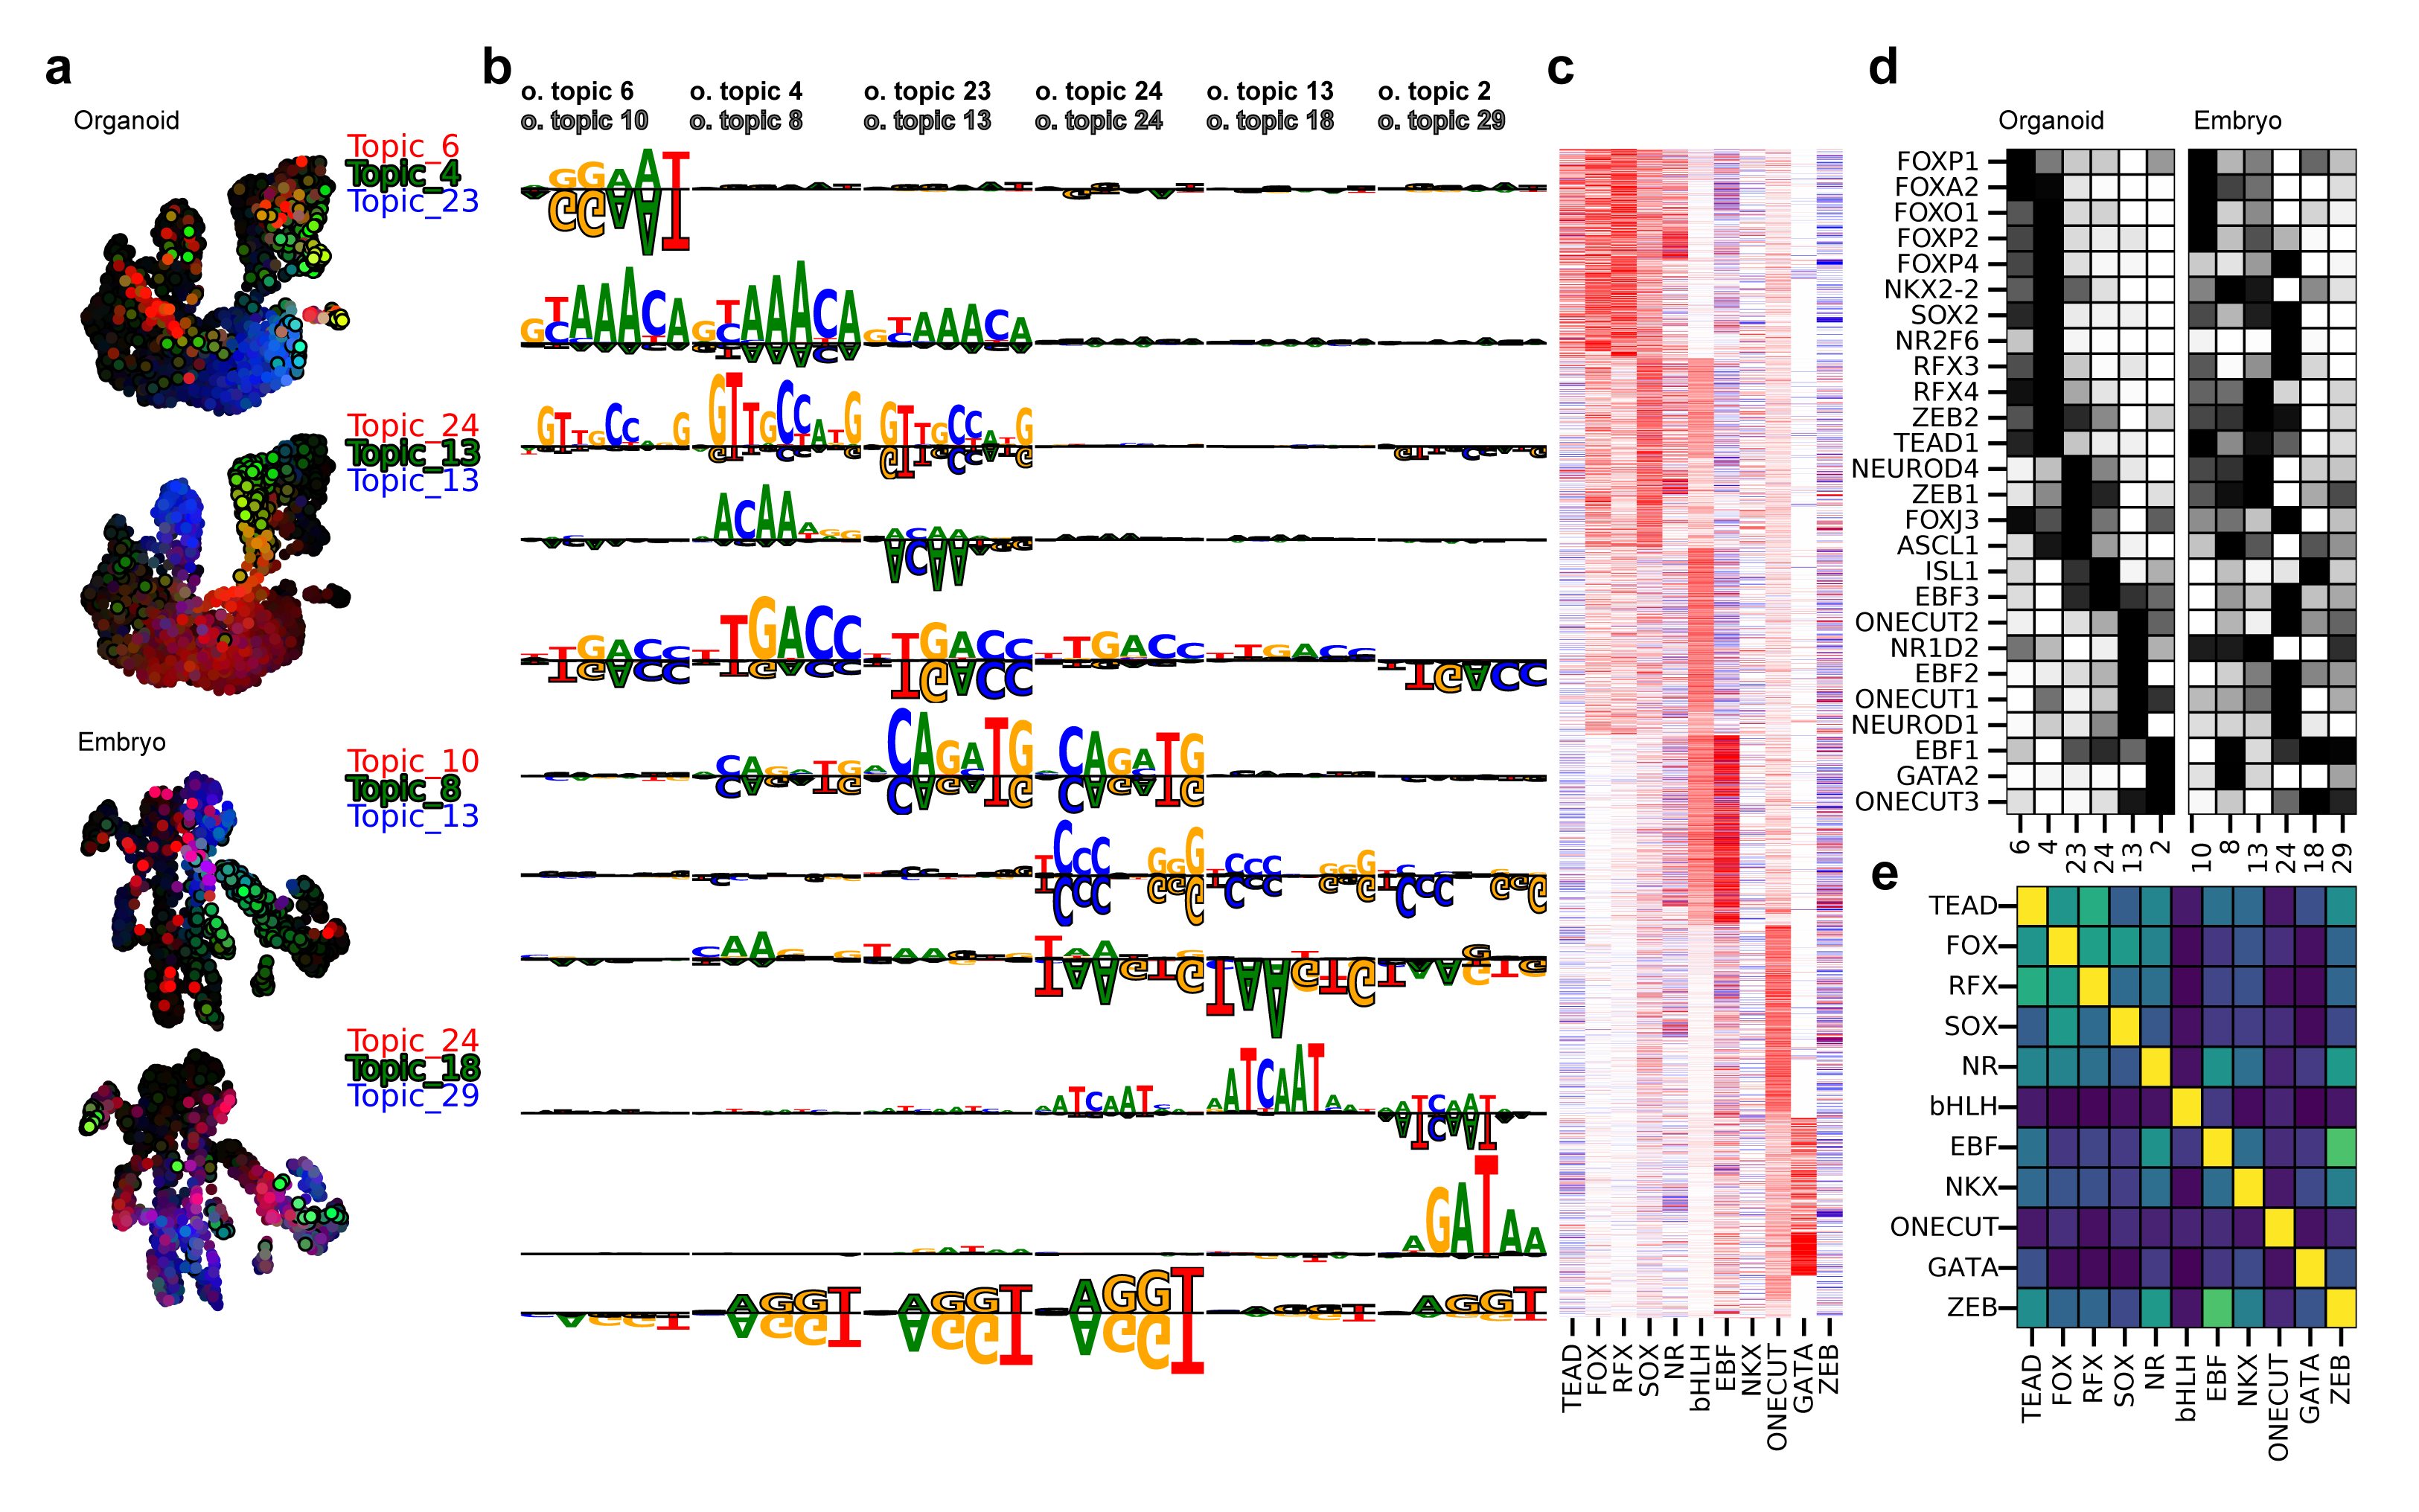
\includegraphics[width=1.0\linewidth]{figures/main/Figure_6.png}

\subsection* {
  Figure 6. Deciphering the enhancer code of early neuronal differentiation.
}

\textbf{a}, UMAP of organoid (top two) and embryo (bottom two) differentiating neuron cells colored by cell-topic probabilities in RGB color scales for neuron related topics. \textbf{b}, Code table showing average contribution score of pattern instances for each neuron related topic. Contribution scores for $DeepNeuralTube_{organoid}$ are not outlined. Contribution scores for $DeepNeuralTube_{embryo}$ are outlined and negated. \textbf{c}, Heatmap showing the maximum normalized contribution score for each of the top 1,000 regions per topic (y-axis) and pattern (x-axis) of neuron related topics. \textbf{d}, Heatmap showing scaled expression of transcription factors corresponding to identified patterns in organoid (left) and embryo (right) for neuon related topics. \textbf{e}, Heatmap showing Jaccard index of regions based on the presence of instances of the identified patterns.


\subsection* {
  Four to five distinct transcription factor binding sites in a region of around 140 base pairs is sufficient to encode
  all cell states related to neuronal progenitors, early neuronal differentiation and neural crest development.
}

Summarizing our results, we identified a total of sixteen and fifteen distinct cell states in respectively the neural
tube organoids and four weeks post conception embryo head with almost one-to-one correspondence based on TFBS importances and TF expression. Additionally, we identified 4 distinct cell states corresponding to AP patterning of the neuronal progenitors in the embryo. To get insight into the minimal set of TFBS that are needed to encode these cell states we trained logistic regression models to classify genomic regions as to belonging to the topic representing each state or not, making use of the motif scores of the identified patterns from each code table (\textbf{Fig. 3e}, \textbf{Fig. 4e}, \textbf{Fig. 5b} and \textbf{Fig. 6b}). The overall performance of these models was acceptably high (\textbf{Fig. 7a}) with an average area under the ROC of X and area under the precision-recall curve of X. Notably, all models for neural crest related states performed best (\textbf{Fig. 7a}). Next, we selected patterns that had a positive coefficient for at least one of the logistic regression models resulting in a total of twenty one patterns for fifteen to sixteen states plus the additional four AP states (\textbf{Fig. 7a}). Finally, we used the identified patterns to design synthetic enhancers for each state using motif embedding\cite{taskiran2024synthetic, kempynck2025crested}. We used at least three TFBS in the design process for each state. In case less than three distinct patterns had a positive coefficient for a state, we implanted multiple copies of each pattern to come to a total of at least four TFBS. The resulting synthetic DNA sequences had an overall high prediction score (X.X on average) (\textbf{Fig. 7a}) - and were cell type specific (\textbf{Fig. 7b}) - with the prediction score for neural crest related states being again the highest. Note that some TFBS like FOX and SOX are used by many cell states (\textbf{Fig. 7a}) while other are more specific to certain states. \par

To conclude, enhancers specific to DV-patterning, neural crest states and early neuronal differentiation tend to be encoded in
the human genome using around four to five distinct TFBS (\textbf{Fig. 7a}) in regions of on average 240-243bp +/- 67-77bp in size (\textbf{Fig. 7c}). AP-patterning enhancers seem to be an exception to this rule, where they are encoded using only two and sometimes even a single TFBS (\textbf{Fig. 7a}).

\noindent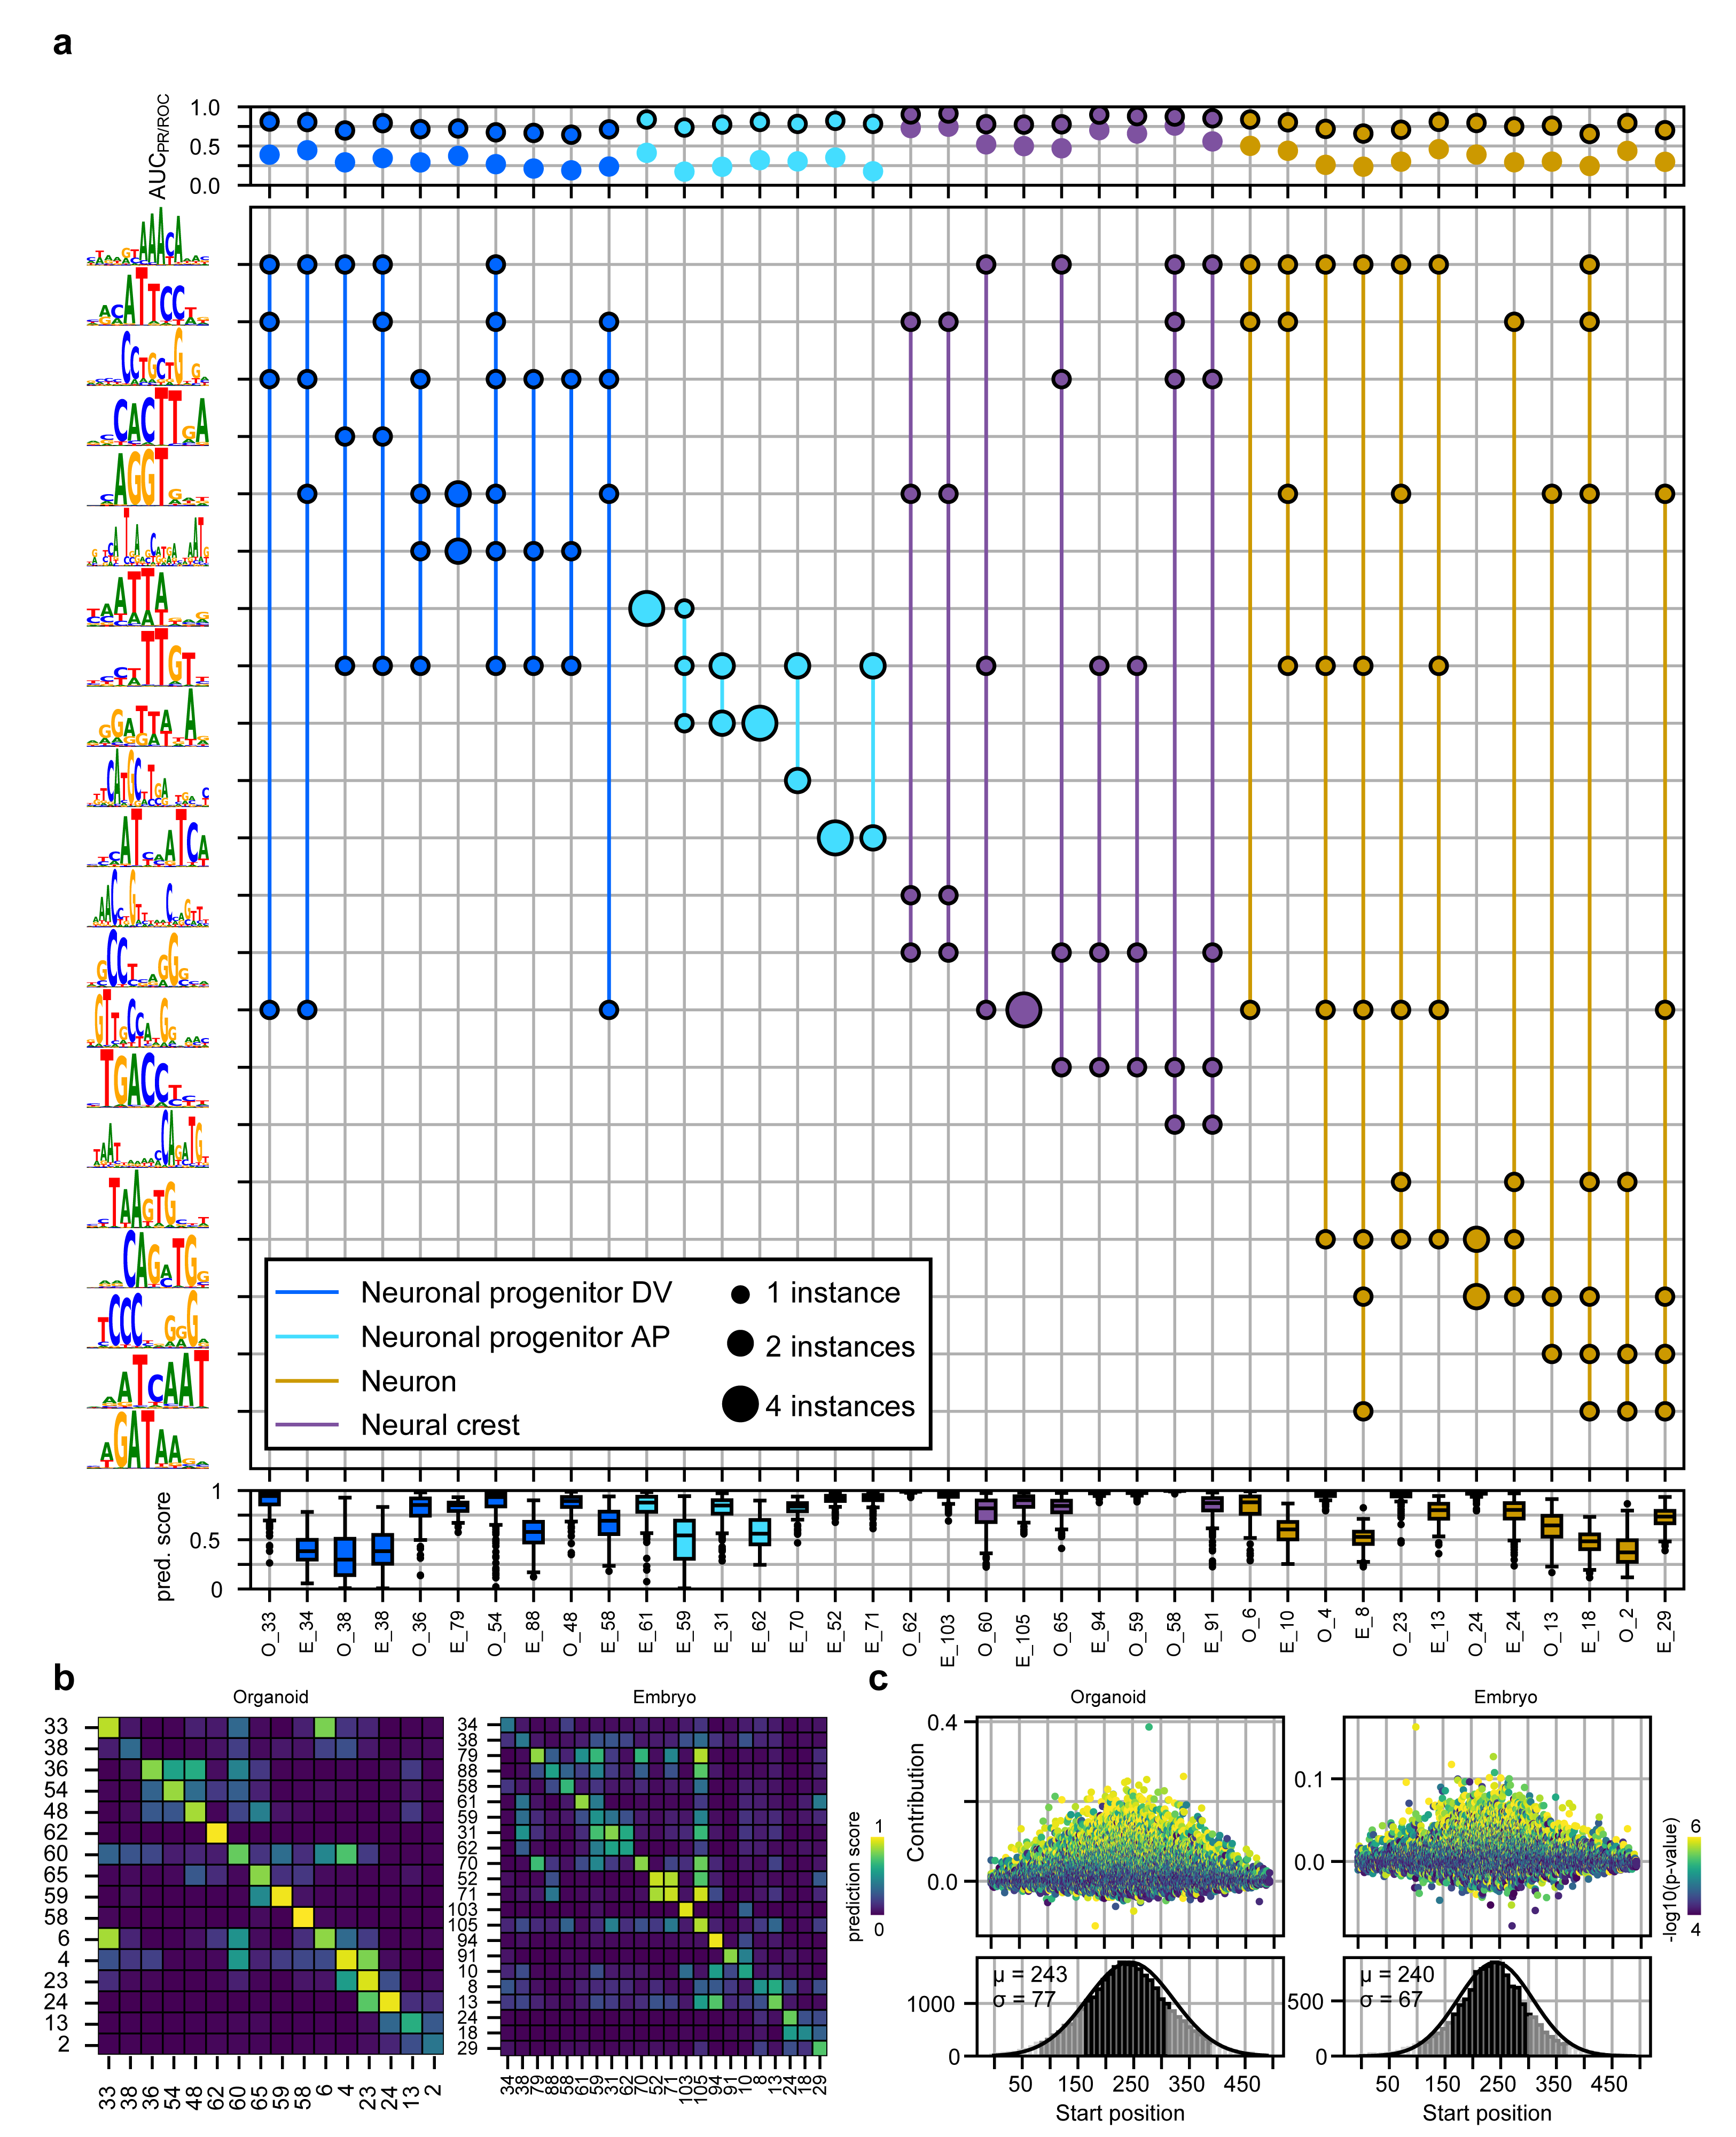
\includegraphics[width=1.0\linewidth]{figures/main/Figure_7.png}

\subsection*{
  Figure 7. Neural tube cell states are encoded using four to five distinct transcription factor binding
  sites
}.
\textbf{a}, Area under the receiver-operator curve (outlined dots) and precision-recall curve of logistic regression
models classifying genomic regions to each topic using motif scores as features (top) and patterns with positive
coefficient for each logistic regression model along with the number of each patterns used for enhancer design
represented by the size of each dot (middle) and boxplots (n = 200) showing prediction score of designed enhancers for
each topic (bottom). \textbf{b}, heatmap showing prediction score for each topic of enhancers designed for all topics
for using $DeepNeuralTube_{organoid}$ (left) and $DeepNeuralTube_{embryo}$ (right). \textbf{c}, scatter plot showing
location of all pattern instances and contribution score at those locations, color is -log p value of the motif score
for each pattern calculated using FIMO\cite{grant2011fimo, schreiber2025tangermeme} for organoid (top left) and embryo
(top right) and histograms showing the number of motif instances per 25 bp bins with confidence intervals indicated in
gray scales (black is +/- 1 standard deviation, gray is +/- 2 standard deviation and white is more than 3 standard
deviations) for organoid (bottom left) and embryo (bottom right).




\section*{DISCUSSION}

%%% The discussion should explain the significance of the results and place them into a broader context.
%%% Subheadings are permitted.

We built an enhancer-code atlas of early human neuronal and neural crest development. Providing enhancer-codes of
neuronal progenitor DV- and AP-patterning, early neuronal fate acquisition and neural crest induction, migration and
facial mesenchyme specification.\par

In order to create this atlas, we generated a single-cell multiome (combined scATAC-seq and scRNA-seq of the same cell) dataset of the head of a four weeks post conception human embryo and we showed that the embryonic cell states can effectively be reproduced using human neural tube organoids on both transcriptomic level and on the level of the enhancer-codes. Specifically, we identified a total of fifteen distinct cell states with one-to-one matches between the organoid and embryo. The fact that cell states were defined in an unbiased manner by making use of topic modeling and that each of these states were independently identified in two separate datasets increases the confidence of their biological relevance. Furthermore, this high similarity between the organoid and the embyro derived cell states validates neural tube organoids as a biological model for early human neural tube and neural crest development, biological cell states that are otherwise not easily accessible in human.\par

The enhancer code remains complicated to study\cite{wassermanAppliedBioinformaticsIdentification2004} especially
compared to the genetic code\cite{kimDecipheringMultiscaleQuantitative2023, deboerHoldOutGenome2024}. Nonetheless, there
are some recurrent patterns that are shared among enhancers of different cell types. In particular, enhancers underlying
DV patterning, early neuronal fate acquisition and neural crest tend to consist out of clusters of 4-5 different
TFBS\cite{kimDecipheringMultiscaleQuantitative2023, longEverChangingLandscapesTranscriptional2016} that are located
within one nucleosome depleted regions (+/-147bp). That is to say, cooperative binding of multiple TFs seem to underlie
the cell type specificity of enhancers\cite{lambertHumanTranscriptionFactors2018}. Here, we see most evidence for a
model of indirect cooperativity\cite{longEverChangingLandscapesTranscriptional2016} (i.e., flexible billboard enhancer
model\cite{arnostiTranscriptionalEnhancersIntelligent2005}). However, for multiple cell types we also observed evidence
of direct coooperativity between TFs in the form of protein-protein interactions between two TFs. This was the case for
TWIST1 and ALX4 heterodimer in facial mesenchyme\cite{kimDNAguidedTranscriptionFactor2024} and GRHL1/2 dimers, TFAP2A and TFAP2B/C  heterodimer\cite{rothsteinHeterodimerizationTFAP2Pioneer2020} and SOX10 homodimers in neural crest. For all these TFs we found dimer motifs with a fixed number nucleotides in between the two TFBS instances. Of note, for SOX10 we observed three different dimer motif with either 3, 4 or 5 bps spacing with those instances with 4 bps spacing being the most accessible (SUPPLEMENT FIG). Finally, we also observed evidence of pioneer activity, where binding of one TF can facilitate the subsequent binding of other TFs to the same enhancer\cite{longEverChangingLandscapesTranscriptional2016}. This was the case for FOXA2 in the floorplate, consistent with previous findings of FOXA TFs\cite{iwafuchi-doiPioneerTranscriptionFactor2016, iwafuchiGeneNetworkTransitions2020}. Others have hypothesized, however, that pioneer activity is not a qualitative feature of a TF but rather dependent on the affinity of interactions between TF and DNA\cite{hansenTestPioneerFactor2022}. Similarly, we observed that FOXA2 binding sites that are specific to the floorplate contain either less FOXA2 binding sites and/or binding sites of lower affinity. The use of suboptimal TFBS is a reoccurring feature of cell type specific enhancers\cite{farleySuboptimizationDevelopmentalEnhancers2015, crockerChapterTwentySevenSoft2016, limAffinityoptimizingEnhancerVariants2024, naqviTransferLearningReveals2025}.

Our results indicate that enhancers underlying neuronal progenitor AP-patterning form an exception to the rule that enhancer
consist out of clusters of 4-5 different TFBS. Homeotypic clusters of 3-4 homeobox instances were sufficient to both create and identify enhancers specific to a certain AP domain. Similar findings were already reported in fly\cite{crockerLowAffinityBinding2015}. It has been a long standing question how homeodomain TFs achieve specific binding\cite{mannChapter3Hox2009, hubertHoxGenesDevelopment2023} given that all homeodomain TFs seem to bind the same \textit{TAAT} motif\cite{bergerVariationHomeodomainDNA2008, noyesAnalysisHomeodomainSpecificities2008}. It has been hypothesized that specificity is mainly achieved through cooperative binding with co-factors\cite{mannChapter3Hox2009}. Indeed, we observe this for EN1 and HOXB3 that are predicted to co-bind with PAX8 and X respectively forming specific dimer motifs. In contrast, we suggest a novel mode where specificity is achieved through the homeodomain itself for TFX and TFY that preferentially bind \textit{TAATTA} and \textit{TAATCC} sites. Thus, additional nucleotides, next to the core \textit{TAAT}, form a TFBS that is both necessary and sufficient for genome wide cell type specificity. In general, although there are only around 100 different DNA binding domains across human TFs\cite{lambertHumanTranscriptionFactors2018} and thus many of the 1,639 known human TFs recognize similar motifs\cite{lambertHumanTranscriptionFactors2018} there are slight variations in preferential TFBS of TFs of the same family\cite{lambertHumanTranscriptionFactors2018, jolmaDNABindingSpecificitiesHuman2013, dealmeidaDeepSTARRPredictsEnhancer2022} that can be important for cell type specific binding.

% single TF
% https://genome.cshlp.org/content/26/7/882.short

%% position of the binding sites vis a vi nucleosomes
% https://www.pnas.org/doi/abs/10.1073/pnas.1804663115

%% Repression through chromatin closing
% carmen paper & ibrahim paper

%% what about repression through chromatin opening

%% clusters of low affinity HOX binding sites
% https://www.cell.com/cell/fulltext/S0092-8674(14)01518-9
% https://elifesciences.org/articles/28975


% another paper of face GWAS: https://www.nature.com/articles/s41588-018-0057-4

% might be interesting
% https://www.nature.com/articles/s41594-024-01449-6
% https://www.nature.com/articles/s41586-018-0549-5

% co-factors (limitation)
% "new" studies
% https://www.biorxiv.org/content/10.1101/2022.08.26.505496v1.abstract
% https://www.cell.com/cell/fulltext/S0092-8674(20)31541-5?uuid=uuid%3A51e14242-dce3-432c-8521-14d9a94b0381
% https://www.cell.com/molecular-cell/fulltext/S1097-2765(21)01070-4?uuid=uuid%3Afbec3fc1-2707-4902-bda8-f196da451272
% https://www.science.org/doi/full/10.1126/science.adf6149
% focus on single enhancers and not entire locus
%
% from lambert et al
%%TFs have traditionally been classified as either ‘‘activators’’ or ‘‘repressors’’; however, this notion has been repeatedly questioned. Many TFs can recruit multiple cofactors that have opposite effects (Frietze and Farnham, 2011; Rosenfeld et al., 2006;
% Schmitges et al., 2016), dependent on the local sequence
%context and availability of cofactors (Meijsing et al., 2009;
%Wong and Struhl, 2011).


% white box models
% DeepNeuralTube
% AP patterning (TP53)
% interpretation of human variation

\subsection*{Limitations of the study}

%%% A "limitations" or "limitations of the study" subsection in the discussion is encouraged and may be required for some
%%% journals and some article formats.

\newpage





\noindent{The following Cell Press journals require most research articles to include their methods in a \textbf{METHODS} section, which should appear after the discussion: \textit{Cell Biomaterials}, \textit{Chem}, \textit{Chem Catalysis}, \textit{Cell Reports Physical Science}, \textit{Cell Reports Sustainability}, \textit{Device}, \textit{Joule}, \textit{Matter}, \textit{Newton}, \textit{One Earth}, and \textit{Patterns}. For all other Cell Press journals, please \textbf{delete} the contents of this page from the template and refer instead to \textbf{STAR Methods} on page 9.}

\section*{METHODS}

%%%  The methods (also/formerly called "experimental 
%%%  procedures") should appear 
%%%  immediately after the discussion. Subheadings 
%%%  may be customized. Please consult your handling 
%%%  editor if you have questions about what content 
%%%  should appear here. 


\subsection*{Custom methods subheading 1}
\subsection*{Custom methods subheading 2}
\subsection*{Custom methods subheading 3}
\subsection*{Custom methods subheading 4}

\newpage






%%%  The following components should appear after the 
%%%  methods. 
%%%  For journals using STAR Methods, these components 
%%%  should appear immediately after the discussion 
%%%  (after any "limitations" or "conclusions" subsection 
%%%  within the discussion).

\section*{RESOURCE AVAILABILITY}

%%%  The resource availability section is required 
%%%  for all research articles. This component 
%%%  has 3 subsections: "lead contact," "materials 
%%%  availability," and "data and code availability." 
%%%  All 3 subsections must be included, even if no 
%%%  unique materials were generated in the study. 
%%%  Do not edit or change the names of the subheadings. 
%%%  No other subheadings or text are allowed in the 
%%%  resource availability section.

\subsection*{Lead contact}

%%%  Authors are required to designate a lead contact, 
%%%  who will be responsible for communication with 
%%%  the journal before and after publication and is 
%%%  the arbiter of disputes, including concerns 
%%%  related to reagents or resource sharing. Only 
%%%  one author can be named the lead contact, and 
%%%  only the lead contact’s information may be 
%%%  provided in this section.

Requests for further information and resources should be directed to and will be fulfilled by the lead contact, Sally White (s.white@university.edu).

\subsection*{Materials availability}

%%%  This subsection must include a statement describing 
%%%  the availability of newly generated materials 
%%%  associated with the paper, including any conditions 
%%%  for access. If there are no newly generated materials 
%%%  associated with the paper, the statement should 
%%%  state this, e.g.: This study did not generate new 
%%%  materials.

Plasmids generated in this study have been deposited to [Addgene, name and catalog number or unique identifier].

\subsection*{Data and code availability}

%%%  All original research papers must include a 
%%%  comprehensive and accurate “data and code 
%%%  availability” statement within the “resource 
%%%  availability” component of the paper before it 
%%%  is accepted for publication. These statements 
%%%  are structured and consist of three bulleted 
%%%  components. Each component must be present.

\begin{itemize}
    \item Small-molecule crystallography data have been deposited at CCDC under the database identifier ABCDEF and are publicly available as of the date of publication. 1H NMR spectra have been deposited at Mendeley under the DOI 10.12345/a1b2c3d4e5f6g7.1 and are publicly available as of the date of publication. All other data reported in this paper will be shared by the lead contact upon request.
    \item All original code has been deposited at Zenodo under the DOI 10.56789/a1b2c3d4e5f6g7.1 and is publicly available as of the date of publication.\cite{georgios_rizos_2023_10253149}
    \item Any additional information required to reanalyze the data reported in this paper is available from the lead contact upon request.    
\end{itemize}


\section*{ACKNOWLEDGMENTS}

%%%  Use this section to acknowledge contributions 
%%%  from non-authors and list funding sources, 
%%%  including grant numbers.

This work was funded by [FUNDER] via grant [GRANT NO.]. The authors thank all members of the lab for their support.

\section*{AUTHOR CONTRIBUTIONS}

%%%  This component is required for most research papers. 
%%%  Mention each individual author with a statement 
%%%  outlining the contribution of each author to the work.

Conceptualization, S.C.P. and S.Y.W.; methodology, A.B., S.C.P., and S.Y.W.; investigation, M.E., A.N.V., N.A.V., S.C.P., and S.Y.W.; writing-–original draft, S.C.P. and S.Y.W.; writing-–review \& editing, S.C.P. and S.Y.W.; funding acquisition, S.C.P. and S.Y.W.; resources, M.E.V and C.K.B.; supervision, A.B., N.L.W., and A.A.D.

\section*{DECLARATION OF INTERESTS}

%%%  This component is required for all articles, even 
%%%  if the authors have no competing interests; if 
%%%  this is the case, insert "The authors declare no 
%%%  competing interests." Please refer to the 
%%%  declaration of interests policy: 
%%%  https://www.cell.com/declaration-of-interests

S.Y.W. is an employee and shareholder of COMPANY. M.E.V. is a founder of COMPANY and a member of its scientific advisory board.

\section*{DECLARATION OF GENERATIVE AI AND AI-ASSISTED TECHNOLOGIES}

%%%  If generative AI and AI-assisted technologies 
%%%  were used in the writing process, this must 
%%%  be disclosed in the paper. This declaration 
%%%  does not apply to the use of basic tools for 
%%%  checking grammar, spelling, references, etc. 
%%%  If you have nothing to disclose, please do not 
%%%  include this component.

During the preparation of this work, the author(s) used [NAME OF TOOL OR SERVICE] in order to [REASON]. After using this tool or service, the author(s) reviewed and edited the content as needed and take(s) full responsibility for the content of the publication.

\section*{SUPPLEMENTAL INFORMATION INDEX}

%%%  Supplemental information must be uploaded as 
%%%  separate files. In the main text, please list the 
%%%  files to be included in a brief index. For details, 
%%%  please review the supplemental information guidelines: 

%%%  Journals with a general "methods" section: 
%%%  http://www.cell.com/supplemental-information

%%%  Journals with STAR Methods: 
%%%  https://www.cell.com/STAR-supplemental-information

\begin{description}
  \item Figures S1-S5 and their legends in a PDF
  \item Table S1. A descriptive title for an Excel file that was too large to appear in the PDF
  \item Table S2. Another descriptive title for a different Excel file
  \item Data S1. Raw data on x, y, and z
\end{description}

\newpage





\section*{MAIN FIGURE TITLES AND LEGENDS}

%%%  At final submission, figure files MUST be 
%%%  provided separately as high-resolution image 
%%%  files. All of the panels for a figure should 
%%%  be in the same file. Figures should have 
%%%  clear labels/file names (Figure 1, Figure 2, 
%%%  etc.). 

%%%  Figure titles and legends should be placed 
%%%  at the end of the main text. You do not 
%%%  need to place the figures, nor their titles 
%%%  and legends, within the main text. While 
%%%  typesetting your article, our team will 
%%%  place each figure in the best location 
%%%  based on the final layout and on your 
%%%  figure citations, e.g., (Figures 1A and 1B). 

%%%  Please review the figure guidelines before 
%%%  submitting your final materials: 
%%%  https://www.cell.com/figureguidelines.

\newpage

\section*{MAIN TABLES, INCLUDING TITLES AND LEGENDS}

%%%  Whenever possible, we encourage you to submit 
%%%  your main-text tables as Microsoft Word documents, 
%%%  using Word's table function. This will ensure 
%%%  the best results during conversion. Tables 
%%%  should be numbered Table 1, Table 2, etc. and 
%%%  should not include subpanels (do not use Table 1A, 
%%%  1B, etc.). Give each table a brief descriptive 
%%%  title. Table legends are optional but encouraged. 
%%%  Footnotes (superscript lowercase letters) should 
%%%  be used where necessary to indicate some feature 
%%%  of the data; please do not use bold, italic, 
%%%  colored text, or shading for this purpose. Use 
%%%  separate cells, not line breaks or spaces, for 
%%%  all discrete data elements. Small embedded 
%%%  graphics with color are OK.

%%%  Like figures, all tables must be cited within 
%%%  the main text, and our typesetting team will 
%%%  place the tables within the typeset paper at 
%%%  the appropriate locations.


\subsection*{Table 1. A table with clear organization of data}

\begin{tabular}{|l | l | l | l|} 
 \hline
 \textbf{Column 1} & \textbf{Column 2} & \textbf{Column 3} & \textbf{Column 4} \\ [1ex] 
 \hline
 Row A\textsuperscript{a} & 6 & 87,837 & 787 \\ [1ex] 
 \hline
 Row B & 7 & 78 & 5,415 \\ [1ex] 
 \hline
 Row C & 545 & 778 & 7507 \\ [1ex] 
 \hline
 Row D & 545 & 18,744 & 7,560 \\ [1ex] 
 \hline
 Row E & 88 & 788 & 6,344 \\ [1ex] 
 \hline
\end{tabular}

\bigskip

The table legend (optional) follows the table itself. The legend should be used to provide additional info that relates to the table as a whole.

\textsuperscript{a}Footnotes can be used to provide additional info on specific content within the table, such as this footnote to the first row (row A). Do not use footnotes in the table title.

\textsuperscript{b}More footnotes

\newpage

%%%  REFERENCES: As of 2023, all Cell Press journals 
%%%  use Numbered (AMA) style. We recommend placing 
%%%  your references in the included "references.bib" 
%%%  file.


\bibliography{references}



\bigskip

%%%  In your References, please include only articles 
%%%  that are published (online publication and 
%%%  preprint servers are OK). Unpublished data, 
%%%  submitted and/or accepted manuscripts, abstracts, 
%%%  and personal communications should be cited within 
%%%  the text only ("unpublished data," "data not 
%%%  shown," "Alice Smith, personal communication") 
%%%  and not included in the references list. Personal 
%%%  communication should be documented by a letter 
%%%  of permission. Whenever possible, please make 
%%%  sure your .bib file has the complete author lists 
%%%  for each item (at minimum, the first 11 authors 
%%%  listed). 

\newpage






All Cell Press \textbf{life and medical science} journals, and the multidisciplinary journal \textbf{iScience}, use the \textbf{\href{https://www.cell.com/star-authors-guide}{STAR Methods}} format for reporting materials and methods. Other Cell Press journals use a non-structured \textbf{methods} format; for those journals, please \textbf{delete} the contents of this page from the template and refer instead to the \textbf{methods} template on page 3.

If you are publishing in a STAR Methods journal, please refer to the appropriate guide for authors:
\begin{itemize}
\item \textit{Cell} authors should download the guide for \textit{Cell} authors \href{https://www.cell.com/pb-assets/journals/research/cell/methods/Methods_Guide_Cell-1678470557763.pdf}{available here}
\item All other journal authors should use \href{https://www.cell.com/pb-assets/journals/research/cell/methods/Methods_Guide_general-1678470557763.pdf}{this version of the guide}
\end{itemize}


\section*{STAR METHODS}

%%%  The STAR Methods should appear in your main 
%%%  manuscript file after the figure legends, main 
%%%  table(s) and table legend(s).

\subsection*{Key resources table}

\textit{To create the KRT, please use the \href{https://star-methods.com}{KRT webform} or the \href{http://www.cell.com/pb-assets/journals/research/cell/methods/table-template1.docx}{Word template} and upload this file separately.}

\subsection*{Experimental model and study participant details}

%%%  Please list here under separate headings 
%%%  all the experimental models/study participants 
%%%  (animals, human participants, plants, microbe 
%%%  strains, cell lines, primary cell cultures) 
%%%  used in the study. For each model, provide 
%%%  information related to their species/strain, 
%%%  genotype, age/developmental stage, sex (and 
%%%  gender, ancestry, race, and ethnicity if 
%%%  reported for human studies), maintenance, 
%%%  and care, including institutional permission 
%%%  and oversight information for the studies 
%%%  the experimental animal/human participant 
%%%  study. The influence (or association) of sex, 
%%%  gender, or both on the results of the study 
%%%  must be reported. In cases where it cannot, 
%%%  authors should discuss this as a limitation 
%%%  to their research’s generalizability.

%%%  Please omit this component if your study does 
%%%  not use experimental models typical in the 
%%%  life sciences (e.g., if your study is 
%%%  computational or physical science research). 

\subsection*{Method details}

%%%  Please provide precise details of all the 
%%%  procedures in the paper (behavioral task, 
%%%  generation of reagents, biological assays, 
%%%  modeling, etc.) such that it is clear how, 
%%%  when, where, and why procedures were 
%%%  performed. We encourage authors to provide 
%%%  information related to the experimental 
%%%  design as suggested by NIH and ARRIVE 
%%%  guidelines (e.g., information about 
%%%  replicates, randomization, blinding, sample 
%%%  size estimation, and the criteria for 
%%%  inclusion and exclusion of any data or 
%%%  subjects).

\subsection*{Quantification and statistical analysis}

%%%  Please describe here all statistical analysis 
%%%  and software used. We ask authors to indicate 
%%%  in this component where all of the statistical 
%%%  details of experiments can be found (e.g., in 
%%%  the figure legends, figures, results, etc.), 
%%%  including the statistical tests used, exact 
%%%  value of n, what n represents (e.g., number 
%%%  of animals, number of cells, etc.), definition 
%%%  of center, and dispersion and precision 
%%%  measures (e.g., mean, median, SD, SEM, confidence 
%%%  intervals). Also, please summarize in this 
%%%  component how significance was defined, the 
%%%  statistical methods used to determine strategies 
%%%  for randomization and/or stratification, sample 
%%%  size estimation, and inclusion and exclusion 
%%%  of any data or subjects, as well as any methods 
%%%  used to determine whether the data met 
%%%  assumptions of the statistical approach.

\subsection*{Additional resources}

%%%  Please provide links to websites that provide 
%%%  further information relevant to the study 
%%%  (e.g., protocol download, troubleshooting 
%%%  forum, etc.). Clinical trial registry numbers 
%%%  and links should also be placed here. Please 
%%%  briefly describe the resource and its 
%%%  relevance for the paper. Please report this 
%%%  information as: “Description: URL.”

Cell.com homepage: https://www.cell.com
\newline Templates for Cell Press authors: https://www.cell.com/article-templates

%%%  ADDITIONAL MANUSCRIPT COMPONENTS:

%%%  Depending on the journal and the article 
%%%  type, you may be asked to upload the 
%%%  following as separate files: graphical 
%%%  abstract, highlights, eTOC blurb (In 
%%%  Brief), and/or other article components 
%%%  such as a "bigger picture" statement. 
%%%  These items are typically not required for 
%%%  initial submissions. Please refer to the 
%%%  journal's website, your acceptance 
%%%  letter, and/or the Final Files 
%%%  Requirements checklist to see if any of
%%%  these items are required (at any stage).


\end{document}
